\documentclass{article}\usepackage[]{graphicx}\usepackage[]{color}
%% maxwidth is the original width if it is less than linewidth
%% otherwise use linewidth (to make sure the graphics do not exceed the margin)

\makeatletter
\def\maxwidth{ %
  \ifdim\Gin@nat@width>\linewidth
    \linewidth
  \else
    \Gin@nat@width
  \fi
}
\makeatother

\usepackage{framed}
\makeatletter

\definecolor{fgcolor}{rgb}{0.345, 0.345, 0.345}
\newcommand{\hlnum}[1]{\textcolor[rgb]{0.686,0.059,0.569}{#1}}%
\newcommand{\hlstr}[1]{\textcolor[rgb]{0.192,0.494,0.8}{#1}}%
\newcommand{\hlcom}[1]{\textcolor[rgb]{0.678,0.584,0.686}{\textit{#1}}}%
\newcommand{\hlopt}[1]{\textcolor[rgb]{0,0,0}{#1}}%
\newcommand{\hlstd}[1]{\textcolor[rgb]{0.345,0.345,0.345}{#1}}%
\newcommand{\hlkwa}[1]{\textcolor[rgb]{0.161,0.373,0.58}{\textbf{#1}}}%
\newcommand{\hlkwb}[1]{\textcolor[rgb]{0.69,0.353,0.396}{#1}}%
\newcommand{\hlkwc}[1]{\textcolor[rgb]{0.333,0.667,0.333}{#1}}%
\newcommand{\hlkwd}[1]{\textcolor[rgb]{0.737,0.353,0.396}{\textbf{#1}}}%



\usepackage{framed}
\makeatletter
\newenvironment{kframe}{%
 \def\at@end@of@kframe{}%
 \ifinner\ifhmode%
  \def\at@end@of@kframe{\end{minipage}}%
  \begin{minipage}{\columnwidth}%
 \fi\fi%
 \def\FrameCommand##1{\hskip\@totalleftmargin \hskip-\fboxsep
 \colorbox{shadecolor}{##1}\hskip-\fboxsep
     % There is no \\@totalrightmargin, so:
     \hskip-\linewidth \hskip-\@totalleftmargin \hskip\columnwidth}%
 \MakeFramed {\advance\hsize-\width
   \@totalleftmargin\z@ \linewidth\hsize
   \@setminipage}}%
 {\par\unskip\endMakeFramed%
 \at@end@of@kframe}
\makeatother

\definecolor{shadecolor}{rgb}{.97, .97, .97}
\definecolor{messagecolor}{rgb}{0, 0, 0}
\definecolor{warningcolor}{rgb}{1, 0, 1}
\definecolor{errorcolor}{rgb}{1, 0, 0}
\newenvironment{knitrout}{}{} % an empty environment to be redefined in TeX

\usepackage{alltt}
\usepackage{fancyhdr}
\pagestyle{fancy}
\setlength{\parskip}{\smallskipamount}
\setlength{\parindent}{0pt}
\usepackage{amsthm}
\usepackage{amsmath}
\usepackage{wrapfig}
\usepackage{graphicx}
\usepackage{float}
\usepackage{caption}
\usepackage{subcaption}
\usepackage[margin=1in]{geometry}
\IfFileExists{upquote.sty}{\usepackage{upquote}}{}

\newtheorem{corollary}{Corollary}[section]
\newtheorem{theorem}{Theorem}
\newtheorem{example}{Example}
\newtheorem{question}{Question}
\newtheorem{remark}{Remark}[section]
\newtheorem{conjecture}{Conjecture}
\newtheorem{proposition}{Proposition}[section]
\newtheorem{definition}{Definition}[section]

\graphicspath{{../figures/}}

\begin{document}


\title{Lab 4-Binary Classifier\\
Stat 215A, Fall 2014}

\author{Andrew Do, Hye Soo Choi, Jonathan Fischer, Xiang (Lisha) Li }

\maketitle

\section{Introduction}
Blah blah...

\section{EDA}

\subsection{Plots of Raw and Expertly Labelled Images}
Figure 1 displays the unprocessed image files for comparison with Figure 2, the expertly-labelled files. With the human eye it is not so difficult to parse cloud from ground based on these images, but we see that cloudy and clear pixels alike run through wide spans of AN so other features must be used.
\begin{figure}[]
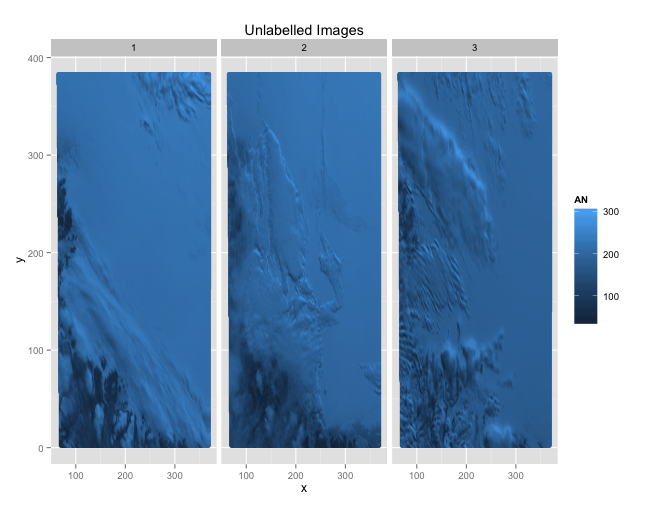
\includegraphics[width = 18cm, height=5cm]{RAWEDA.png}
\caption{Raw images with AN radiances.}
\end{figure}

\begin{figure}[]
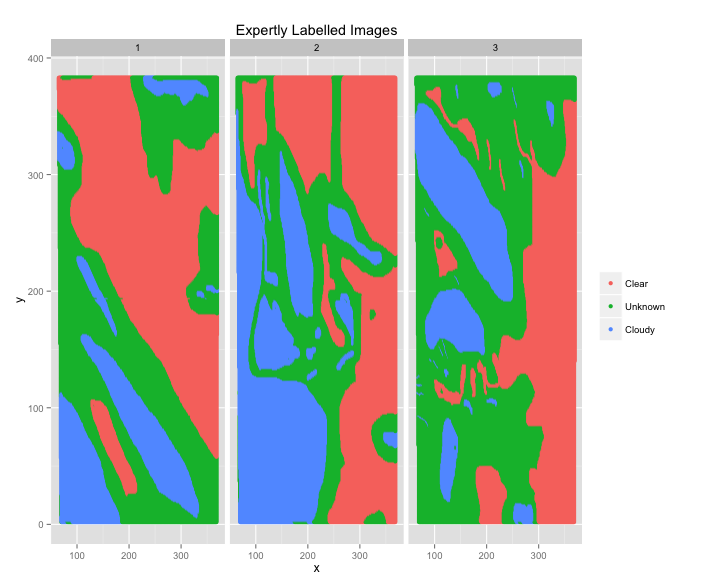
\includegraphics[width = 18cm, height=5cm]{EXPERTSEDA.png}
\caption{Images with expert classifications. Proportions: 39.8$\%$ unknown, 23.4$\%$ cloudy, 36.8$\%$ clear.}
\end{figure}
\subsection{Densities of NDAI, SD and CORR}

The following three plots gives us a sense of what can be learned from NDAI, SD and CORR.  The densities are grouped by their expert labels, red is for `no cloud', green are for `unknown' and blue for `cloud'. We can see that NDAI has reasonably good separation between cloud and no cloud, in all three pictures, which is confirmed in our later modeling sections by Gini importance measures found in the random forest model and it's importance as a variable in LDA/QDA and logit models. In comparison, SD does not have as  good of a separation within the smaller SD values, however it is still clear that pixels labelled as clouds are the only pixels with higher SD values.  We thus expect the two features in combination can help determine whether a pixel with high NDAI should be labelled as a cloud by using the SD feature.  Finally CORR values appear to be a good separator for image 2, but much less so for image 1.  This uneven distribution of CORR values between images prompted us to cross validate our models across images, in addition to the folds created by dividing each image into 4 quadrants. 

\begin{figure}[H]
\minipage{0.32\textwidth}
  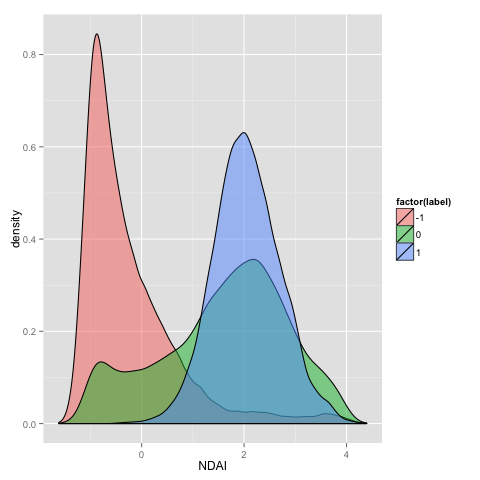
\includegraphics[width=\linewidth, height = 100pts ]{NDAI1.png}
\endminipage\hfill
\minipage{0.32\textwidth}
  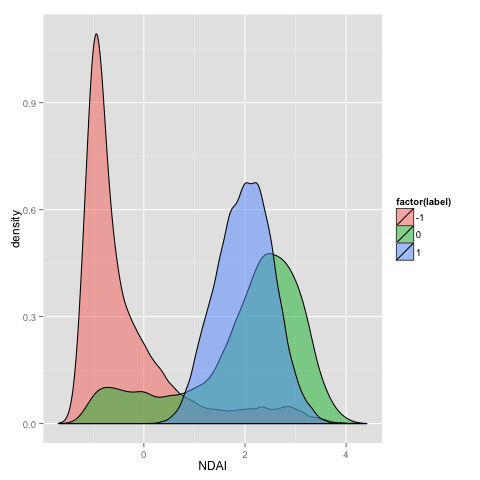
\includegraphics[width=\linewidth, height = 100pts]{NDAI2.png}
\endminipage\hfill
\minipage{0.32\textwidth}%
  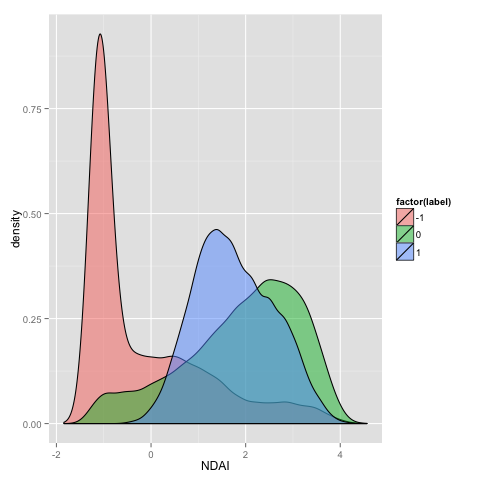
\includegraphics[width=\linewidth, height = 100pts]{NDAI3.png}
\endminipage
  \caption{NDAI density plot for Image 1, 2, 3 (respectively).}\label{}
\end{figure}

\begin{figure}[H]
\minipage{0.32\textwidth}
  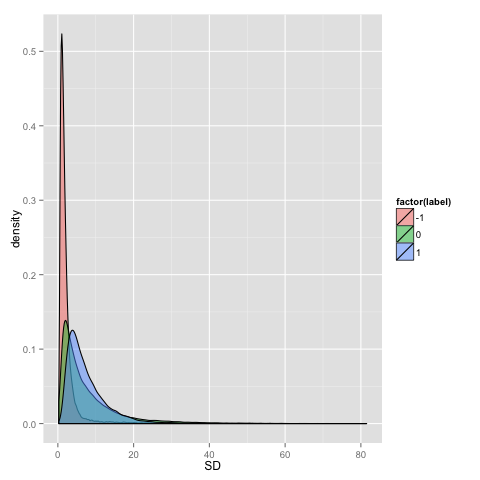
\includegraphics[width=\linewidth, height = 100pts]{SD1.png}
\endminipage\hfill
\minipage{0.32\textwidth}
  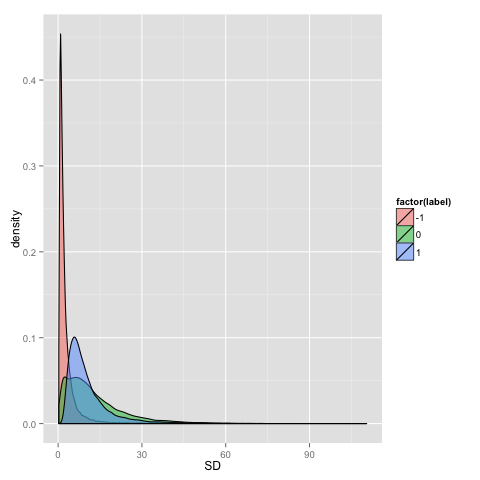
\includegraphics[width=\linewidth, height = 100pts]{SD2.png}
\endminipage\hfill
\minipage{0.32\textwidth}%
  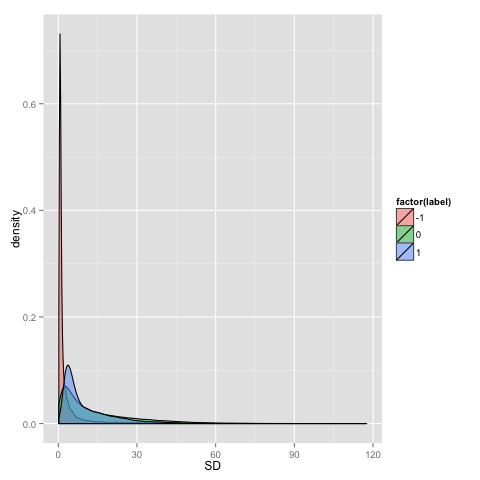
\includegraphics[width=\linewidth, height = 100pts]{SD3.png}
\endminipage
  \caption{SD density plot for Image 1, 2, 3 (respectively).}
\end{figure}

\begin{figure}[H]
\minipage{0.32\textwidth}
  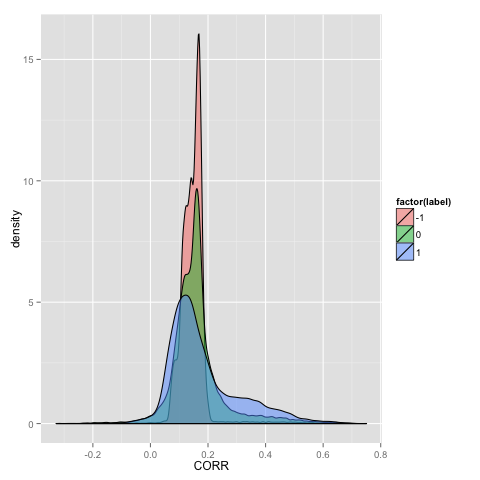
\includegraphics[width=\linewidth, height = 100pts]{CORR1.png}
\endminipage\hfill
\minipage{0.32\textwidth}
  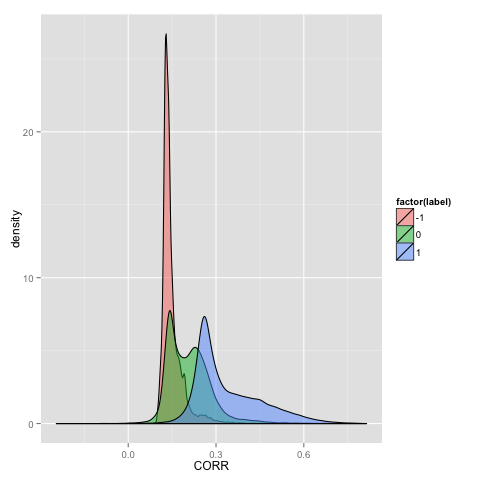
\includegraphics[width=\linewidth, height = 100pts]{CORR2.png}
\endminipage\hfill
\minipage{0.32\textwidth}%
  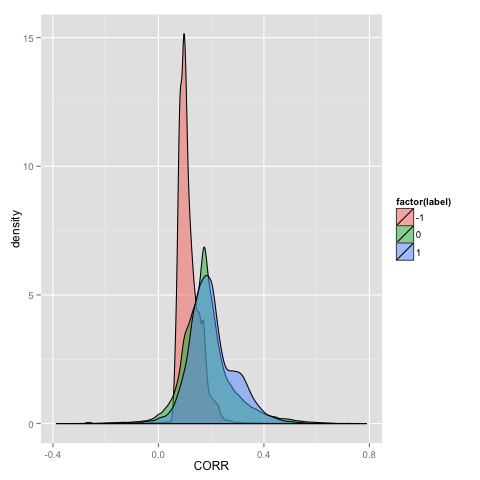
\includegraphics[width=\linewidth, height = 100pts]{CORR3.png}
\endminipage
  \caption{CORR density plot for Image 1, 2, 3 (respectively).}\label{}
\end{figure}


\begin{figure}[h]
  \centering 
  \begin{subfigure}[b]{0.3\textwidth}
    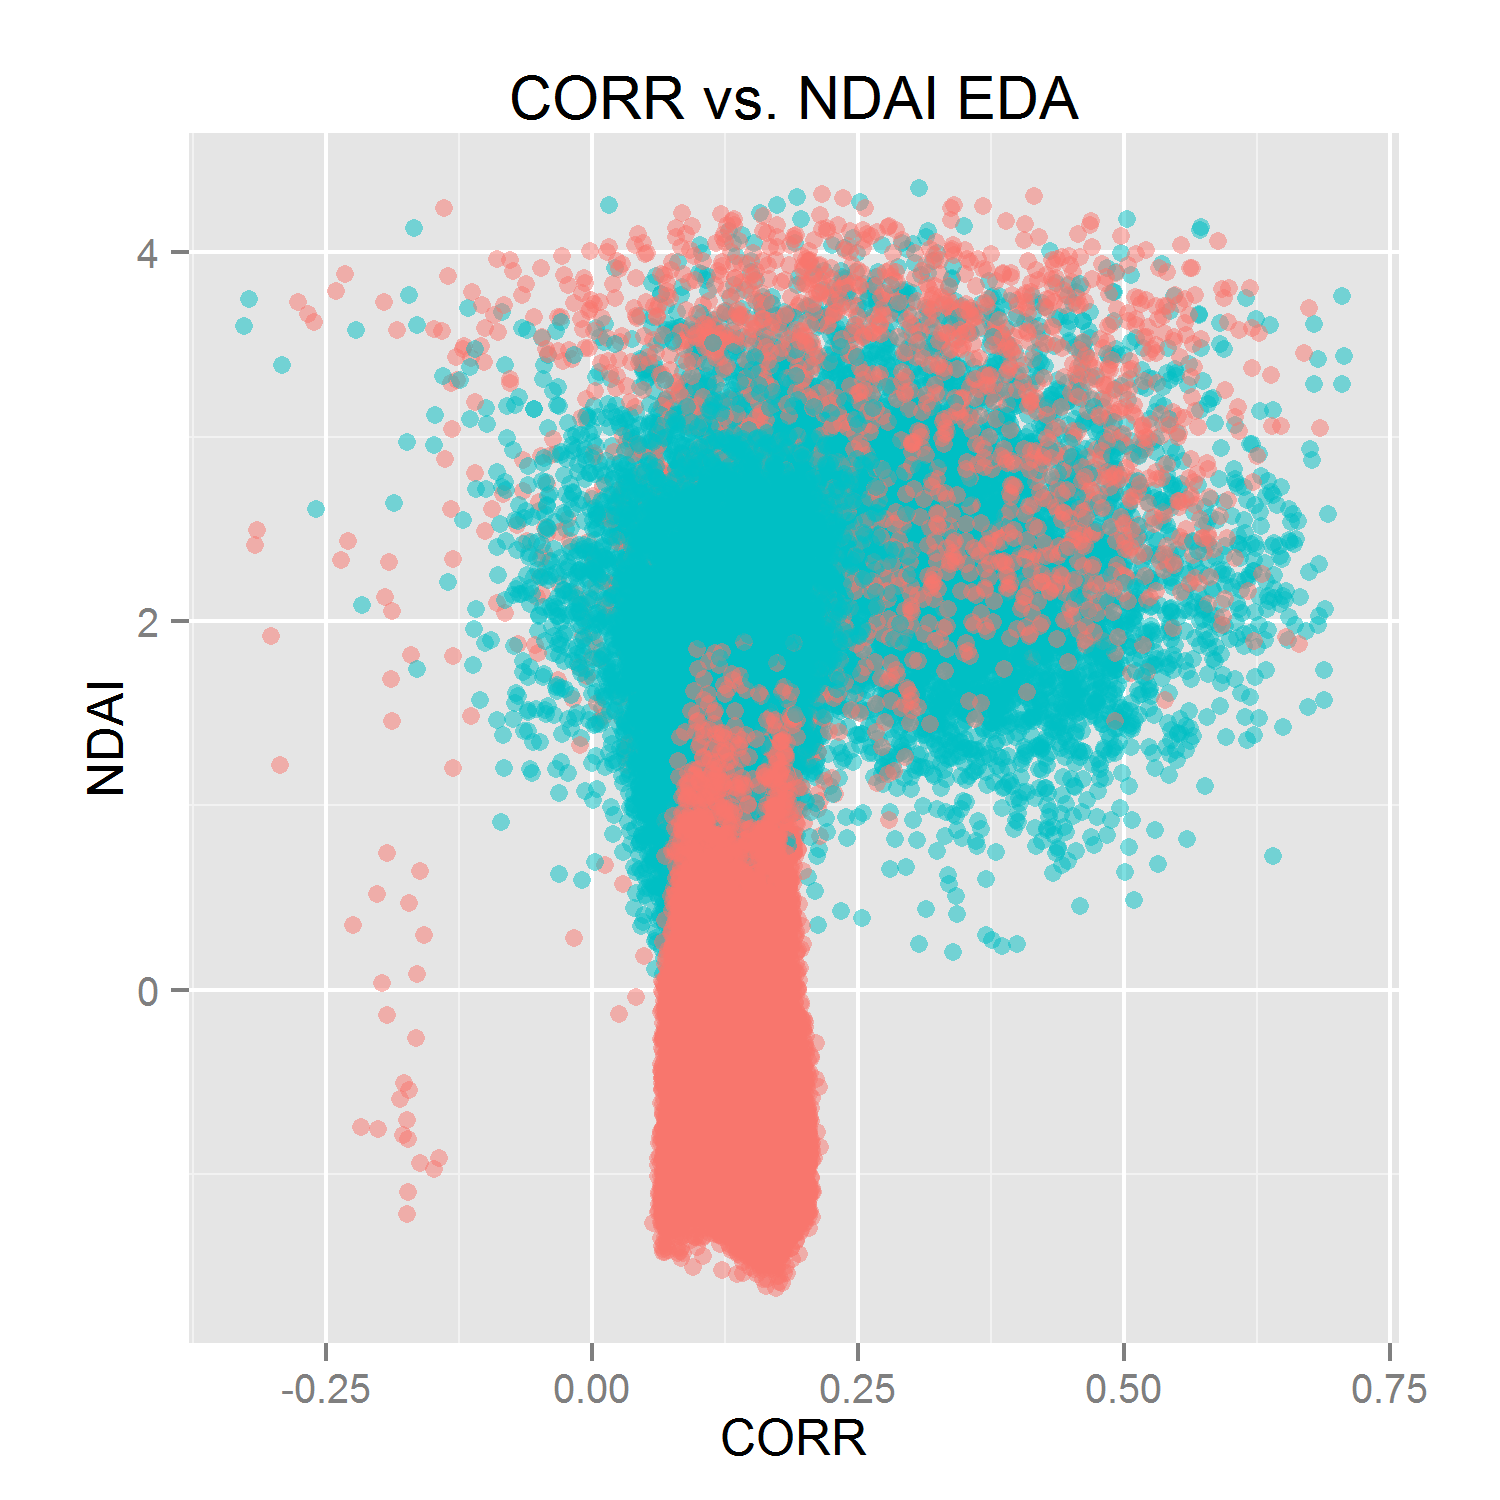
\includegraphics[width=\linewidth]{CORR_vs_NDAI.png}
    \caption{CORR vs. NDAI Plot of Image 1}
    \label{CorrNdai}
  \end{subfigure} 
  \begin{subfigure}[b]{0.3\textwidth}
    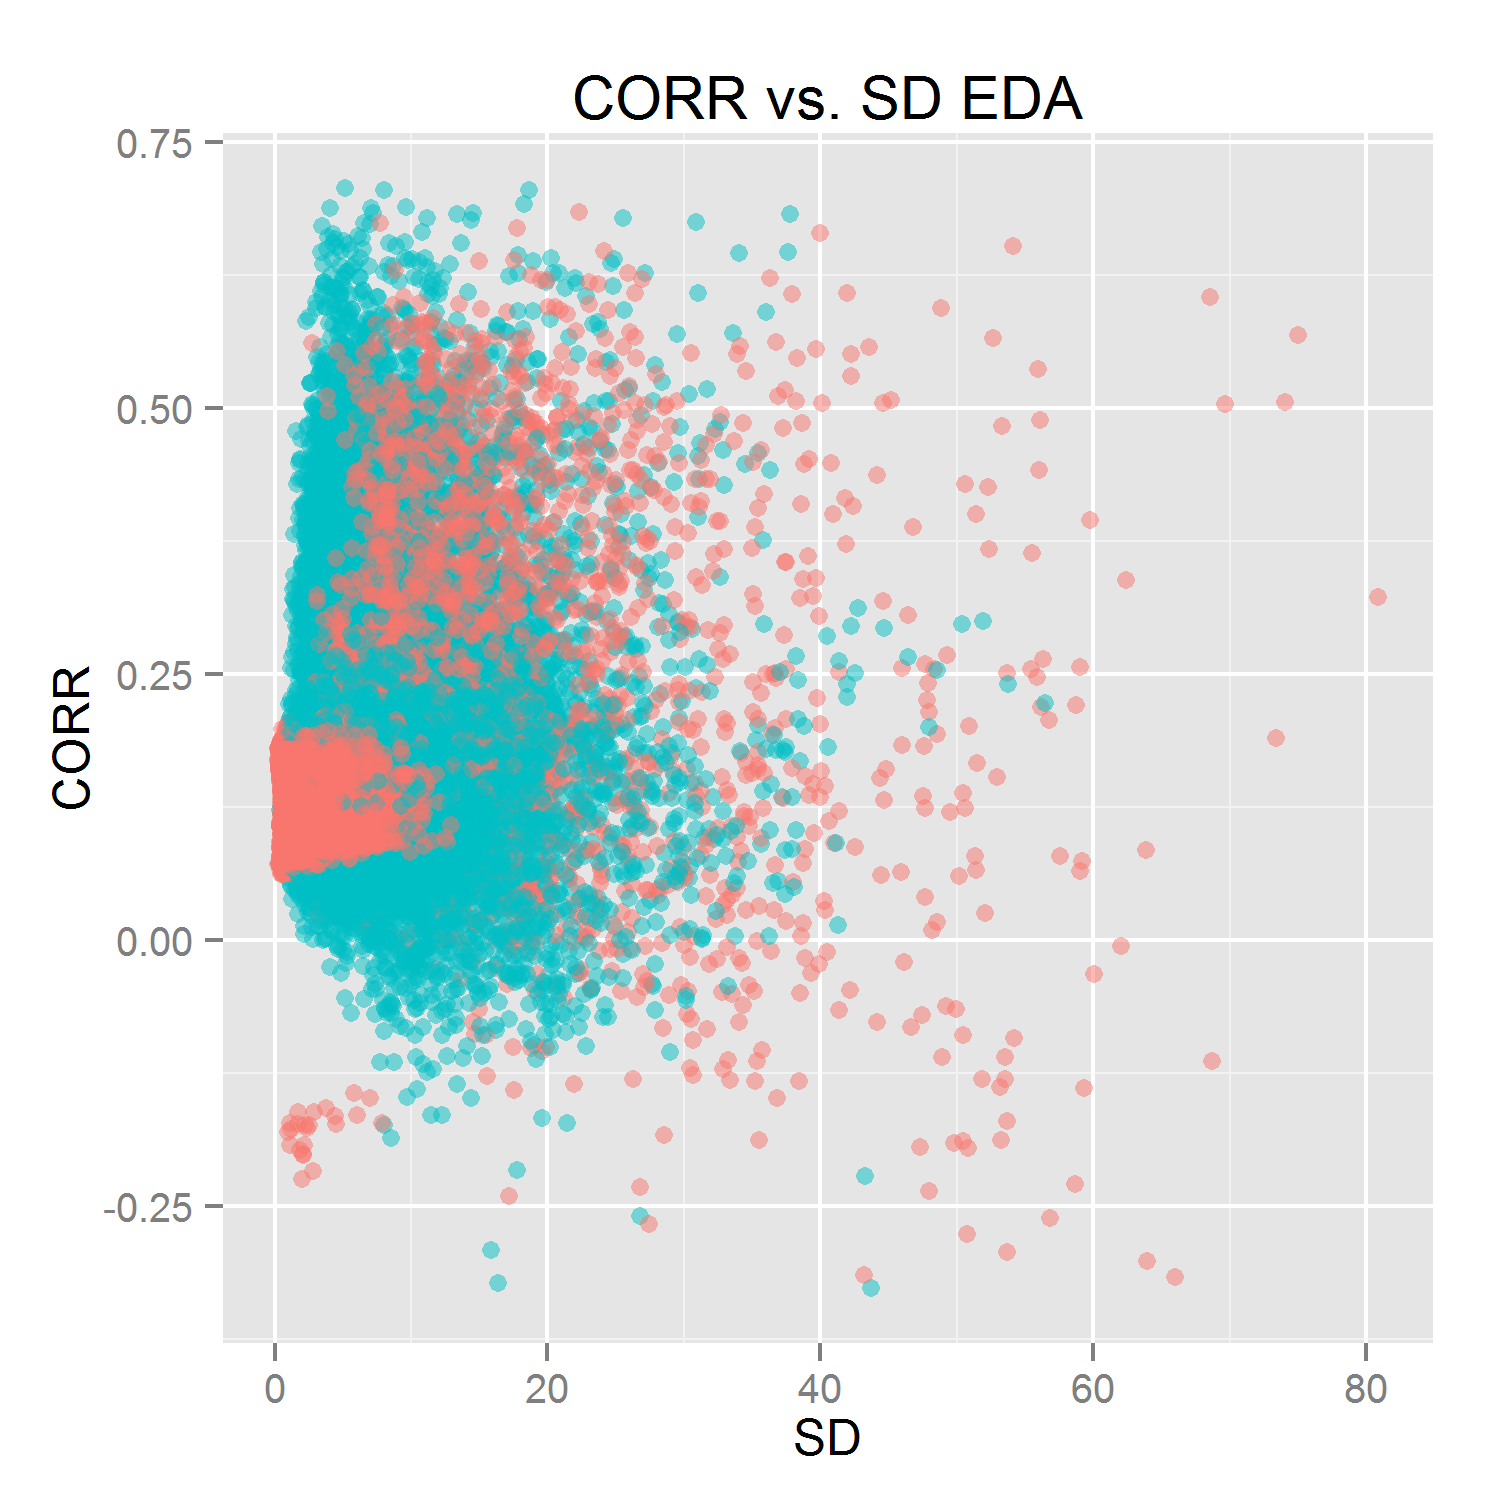
\includegraphics[width=\linewidth]{CORR_vs_SD.png}
    \caption{CORR vs. SD Plot of Image 1}
    \label{CorrSd}
  \end{subfigure}  
  \begin{subfigure}[b]{0.3\textwidth}
    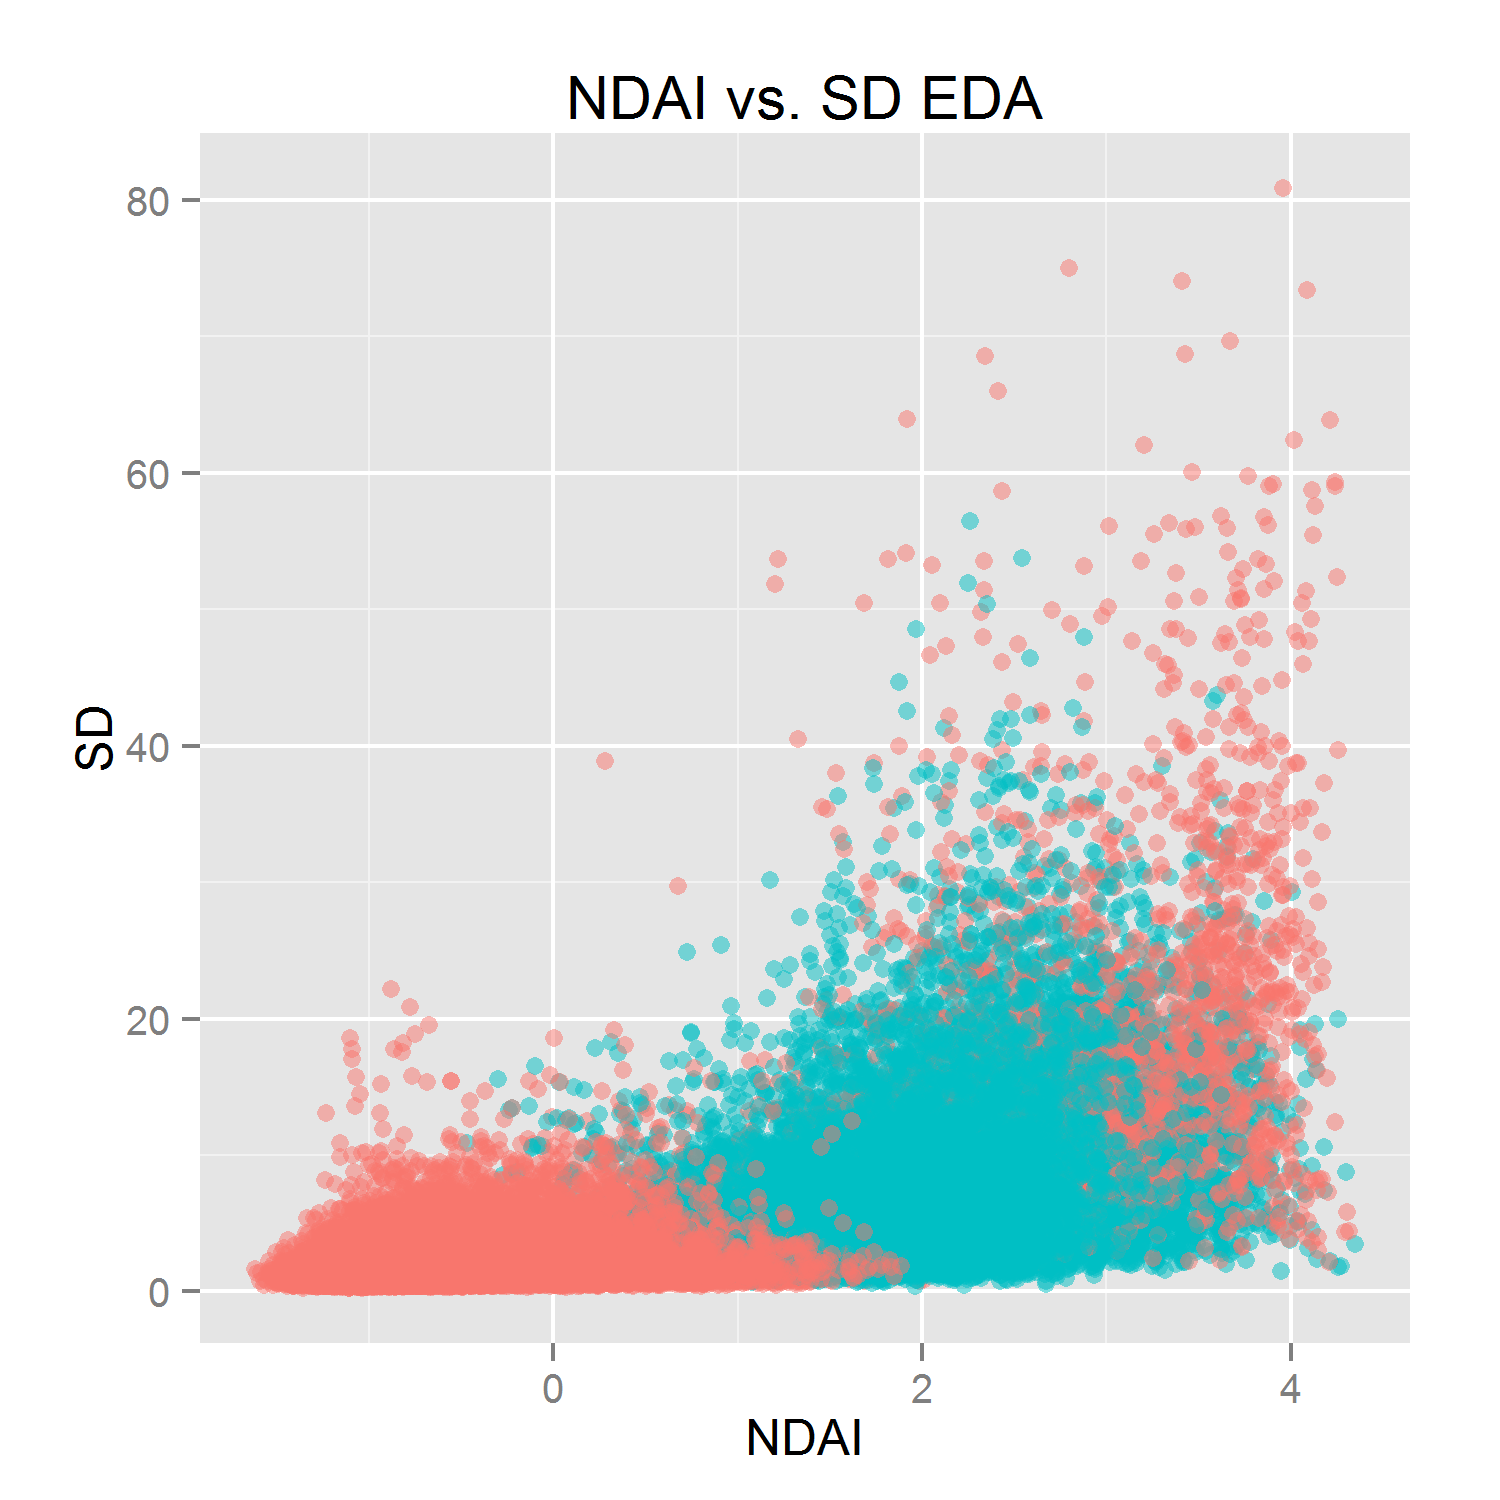
\includegraphics[width=\linewidth]{NDAI_vs_SD.png}
    \caption{NDAI vs. SD Plot of Image1}
    \label{NdaiSd}
  \end{subfigure}
  \caption{Scatter plots of the pairs of features used in the analyses. Red points denote pixels that were labeled as not clouds and blue points represent cloudy pixels.}
  \label{fig:Scatter}
\end{figure}
Figure \ref{fig:Scatter} shows hope that our selected features may be able to distinguish between cloudy and icy pixels.  The rounded boundaries suggest that non-linear surfaces may be necessary to separate the feature space.

\subsection{Mapped Features}
The ensuing figures plot the engineered feature values (NDAI, SD, CORR) spatially. In agreement with the NDAI density plots, higher NDAI values indicate increased likelihood of the presence of clouds, and the NDAI plots look quite similar to the binary classification plots. The SD maps show areas of high variance in the radiances thereby providing a decent outline of cloud boundaries. Unfortunately, this can also lead to the highlighting of uneven ground regions. Finally, the CORR images resemble weakened versions of their NDAI counterparts though with some additional strange behavior in the bottom left corners of Images 1 and 2. 
\begin{figure}[H]
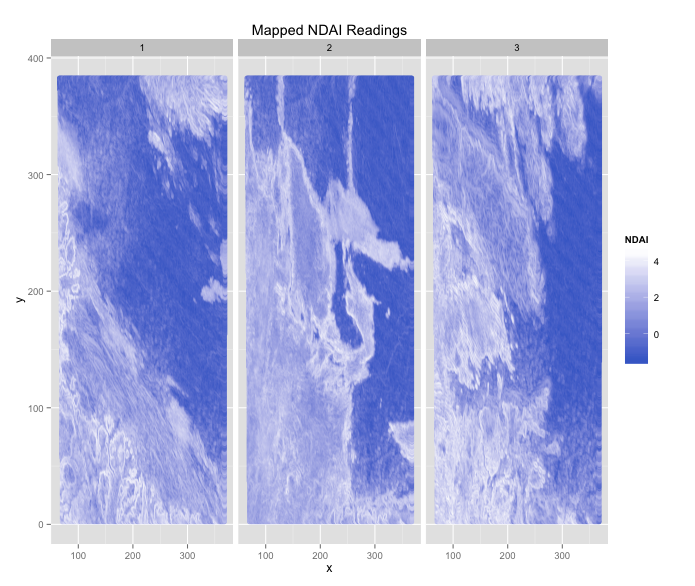
\includegraphics[width = 18cm, height = 5cm]{NDAIEDA.png}
\caption{Mapped NDAI readings. We see good correspondence between larger values and presence of clouds.}
\end{figure}

\begin{figure}[H]
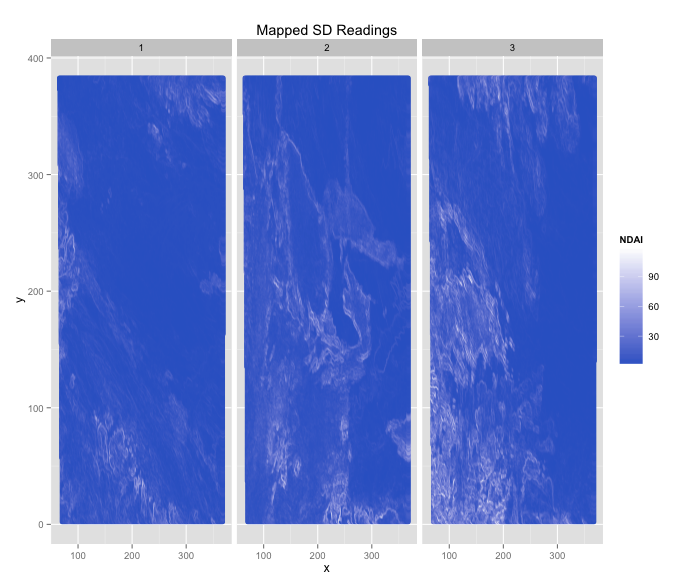
\includegraphics[width = 18cm, height = 5cm]{SDEDA.png}
\caption{Mapped SD readings. Higher values show cloud boundaries, though also show uneven terrain.}
\end{figure}

\begin{figure}[H]
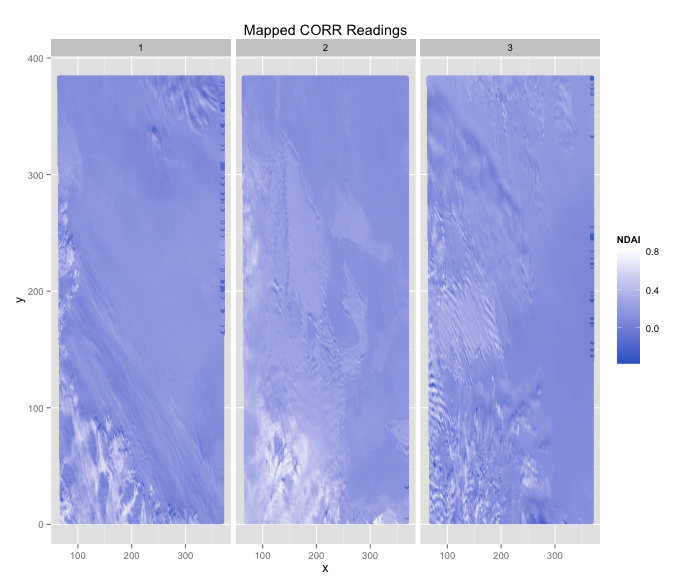
\includegraphics[width = 18cm, height = 5cm]{CORREDA.png}
\caption{Mapped CORR readings. Cloudy regions tend to be lighter, but not as strongly as in NDAI.}
\end{figure}

\section{Modeling}

\subsection{QDA/LDA}

\begin{figure}[h]
  \centering 
  \begin{subfigure}[b]{0.3\textwidth}
    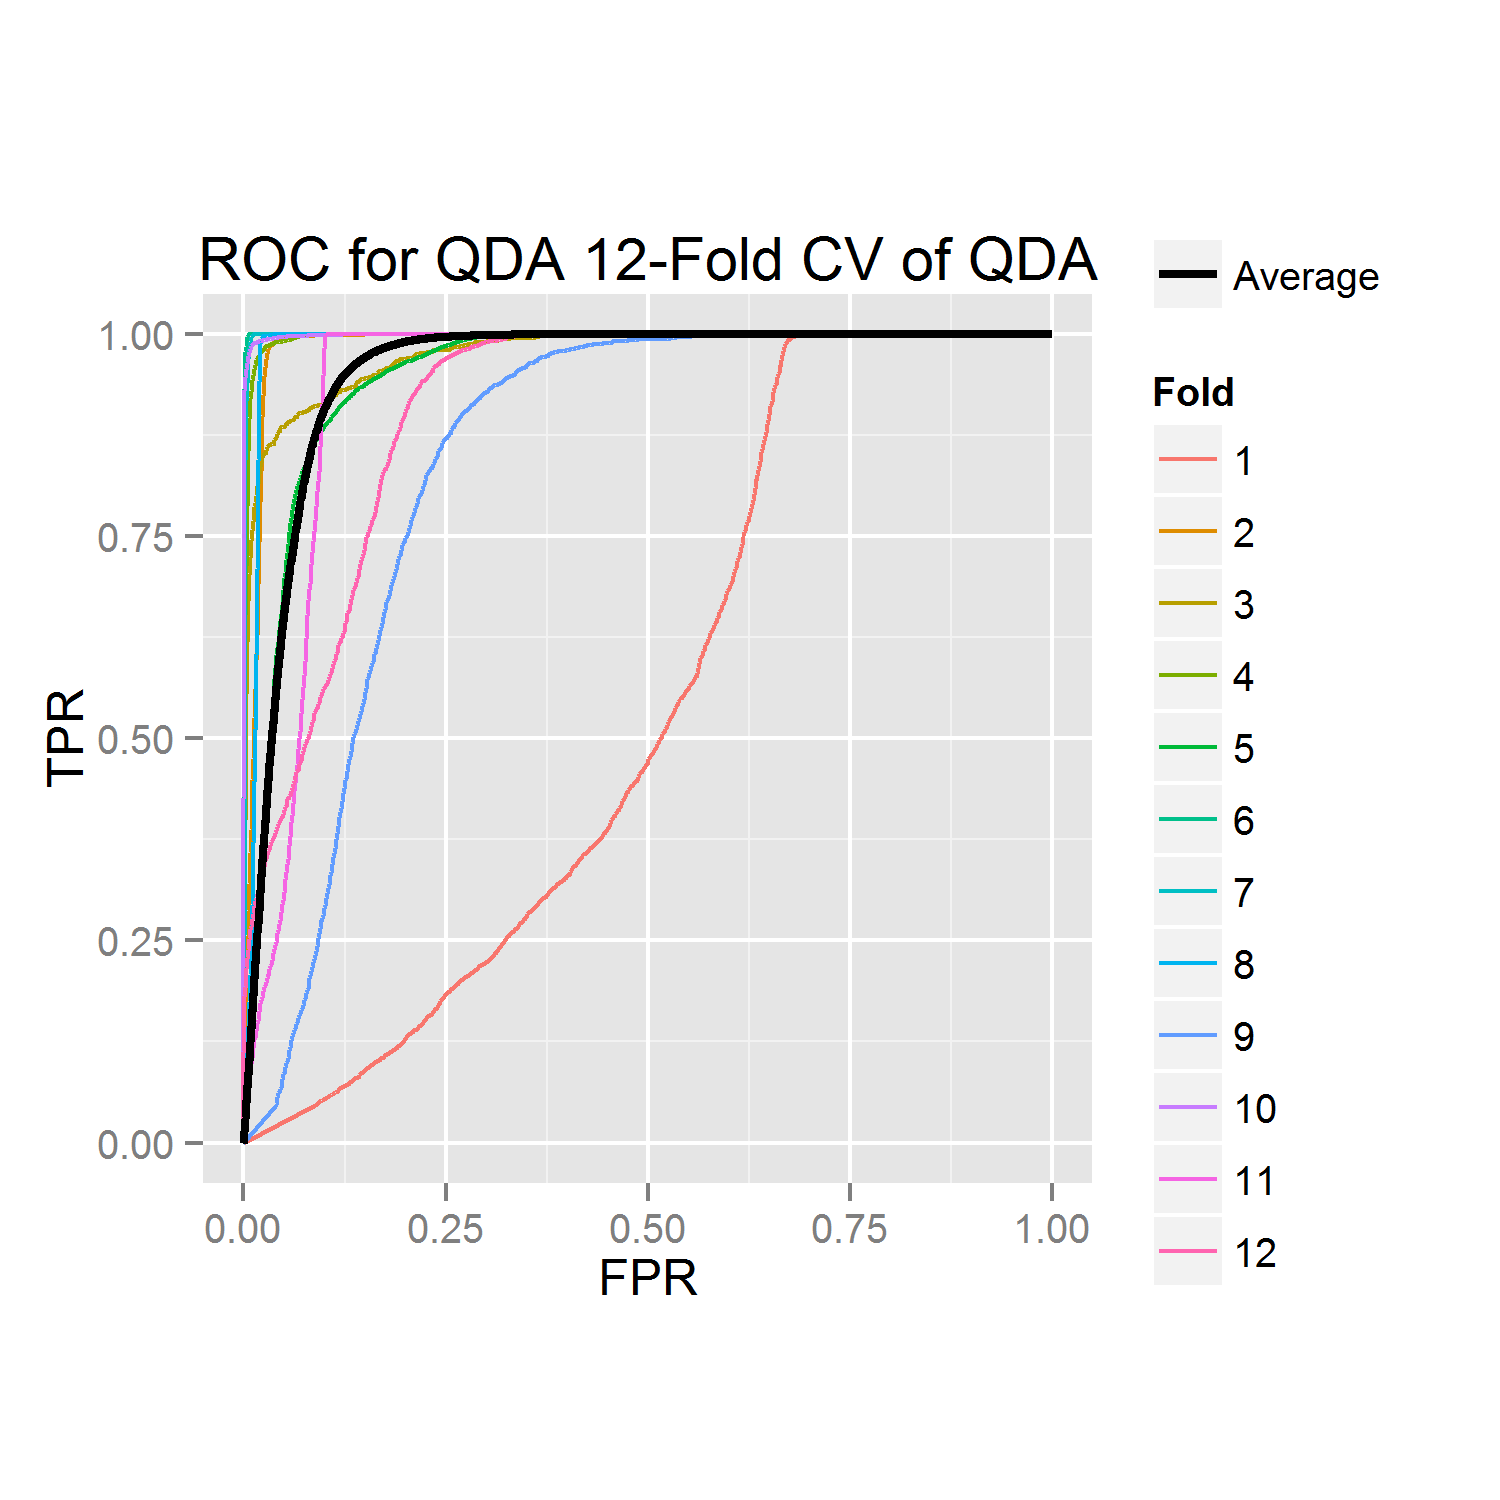
\includegraphics[width=\linewidth]{ROC_12_folds_DA.png}
    \caption{ROC for 12-fold CV of QDA}
    \label{12-foldROC}
  \end{subfigure}  
  \begin{subfigure}[b]{0.3\textwidth}
    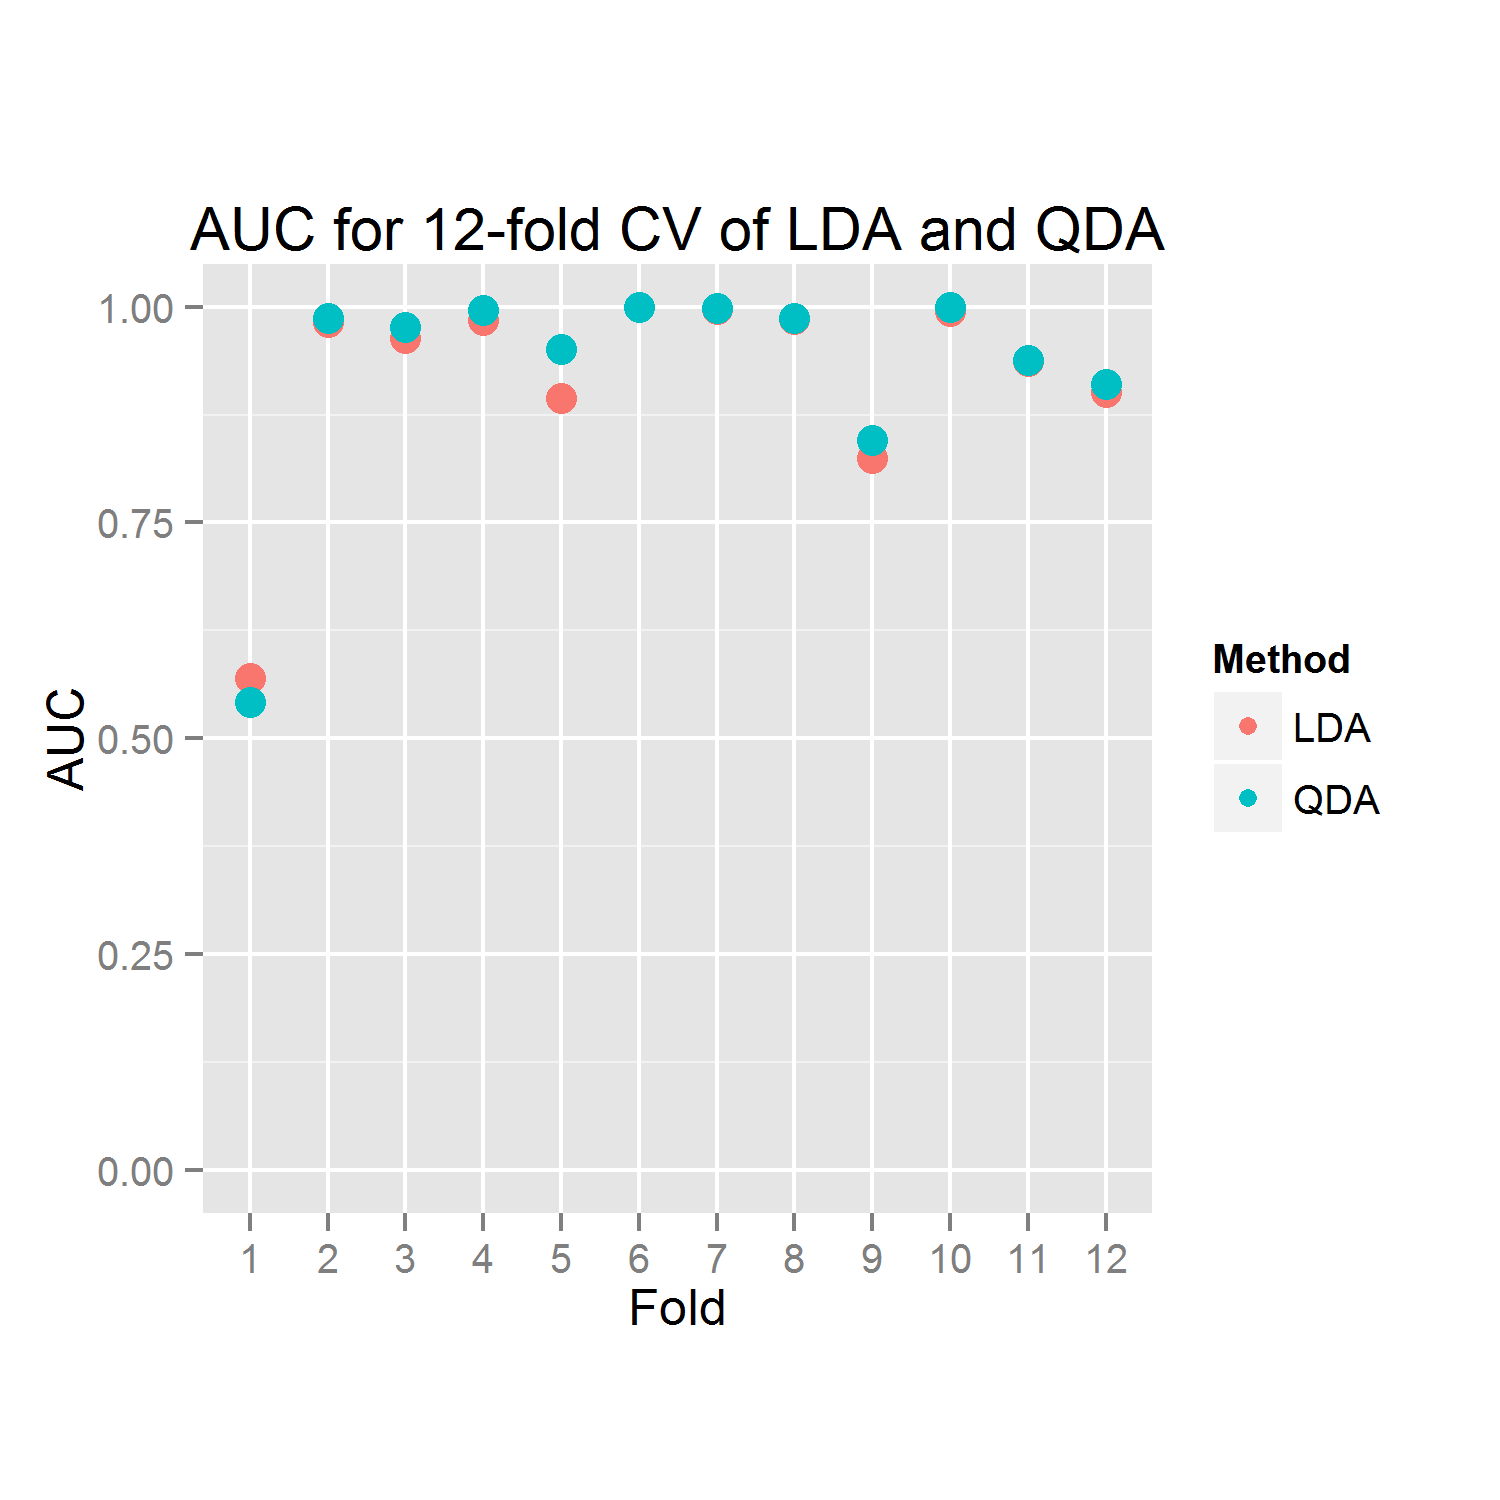
\includegraphics[width=\linewidth]{AUC_12_folds_DA.png}
    \caption{AUC for LDA QDA Classifiers}
    \label{12-foldAUC}
  \end{subfigure}  
  \begin{subfigure}[b]{0.3\textwidth}
    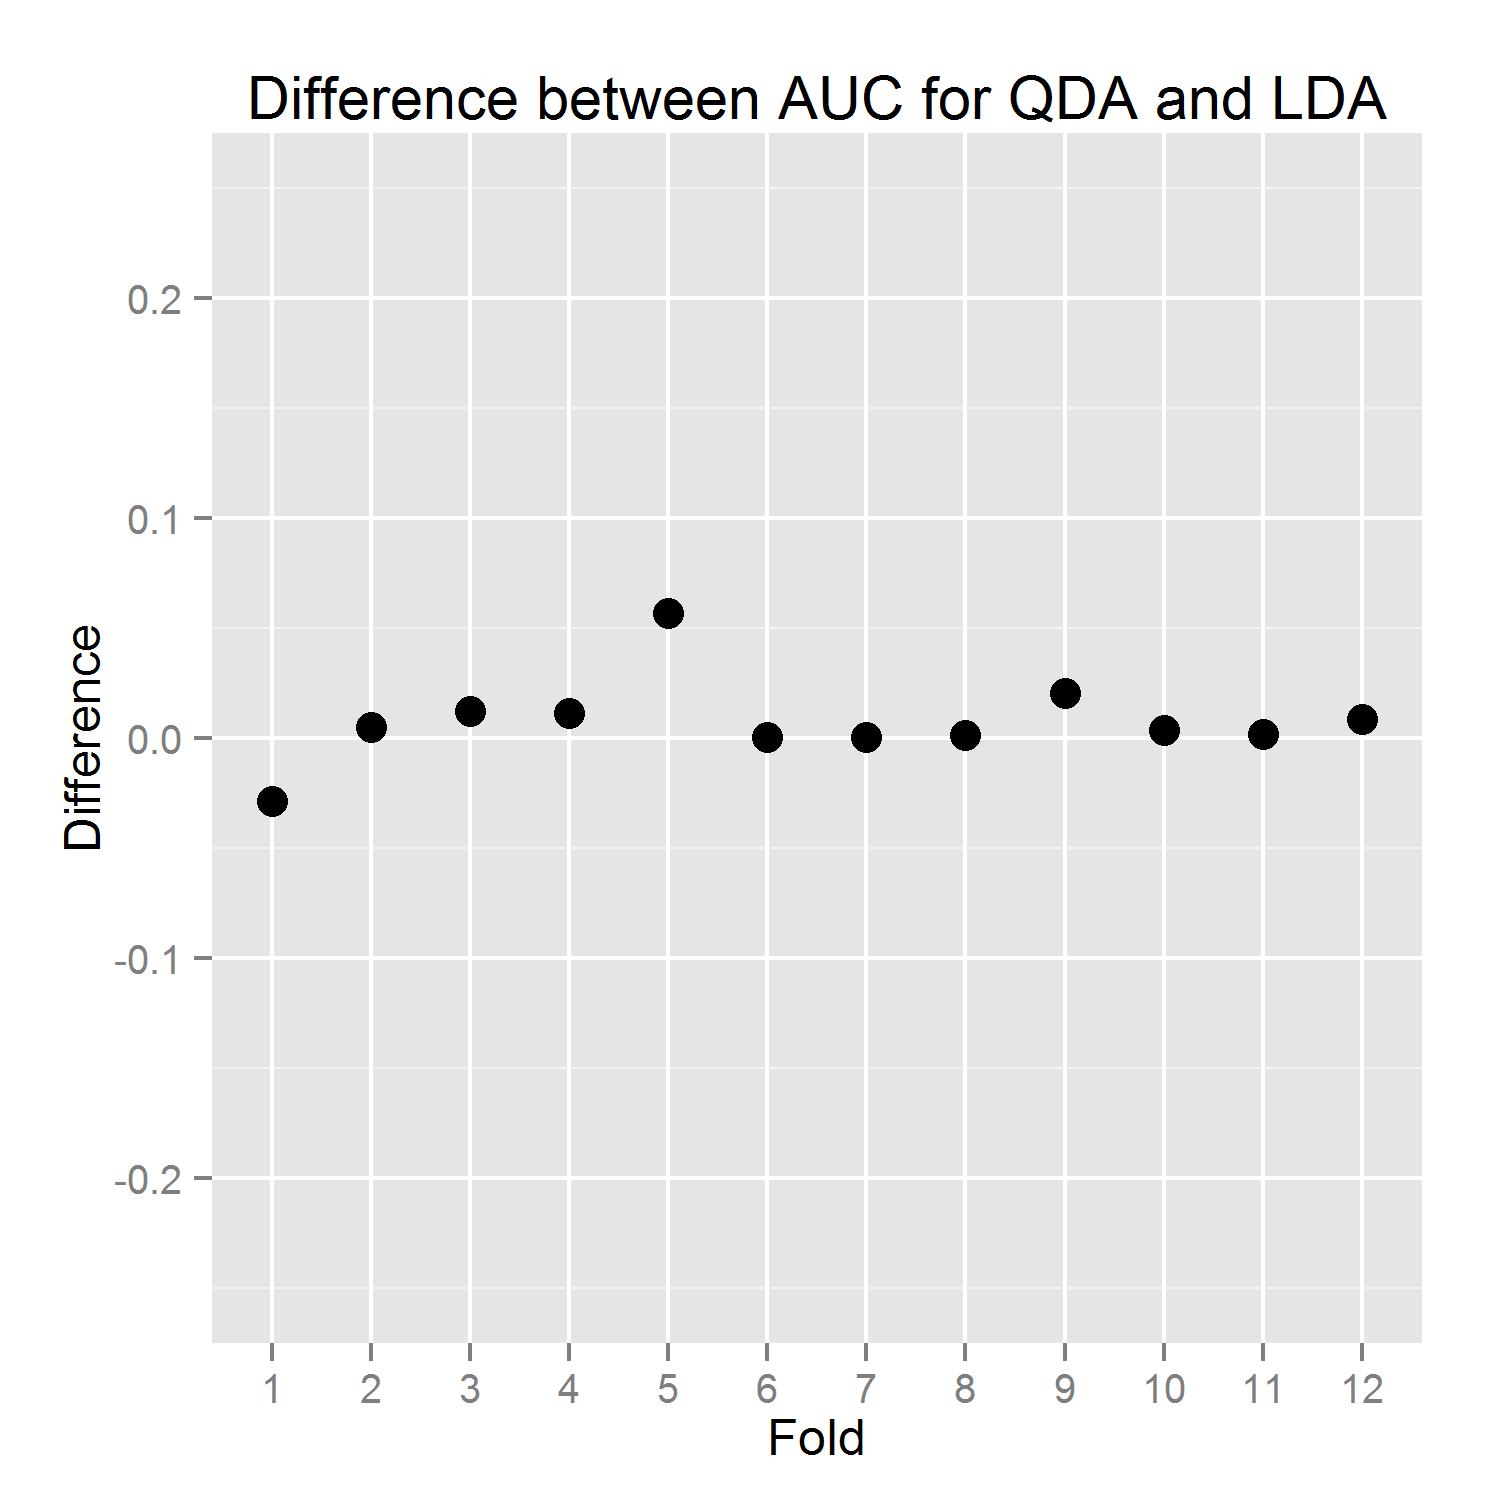
\includegraphics[width=\linewidth]{AUC_difference.png}
    \caption{AUC Differences}
    \label{12-foldAUCdiff}
  \end{subfigure}    
  \caption{(\ref{12-foldROC}) shows the ROC curves for each of the 12 folds of cross validation.  (\ref{12-foldAUC}) and (\ref{12-foldAUCdiff}) show evidence via AUC estimates that QDA performs slightly better than LDA.  Note that in both analysis, fold 1 has an abnormally low AUC.}
  \label{fig:qda_lda}
\end{figure}
Linear discriminant analysis (LDA) for binary classification aims to separate the feature space using a hyperplane.  It assumes that the each class is normally distributed with means $\mu_0$ and $\mu_1$ and that the two classes are homoscedastic with covariance matrix $\Sigma_0=\Sigma_1=\Sigma$.  Quadratic discriminant analysis works in the same manner except that it makes no assumptions about the covariance matrix.  Thus given the multivariate Guassian distribution:
\begin{equation}
f_c(x) = \frac{1}{(2 \pi)^{p/2} \vert \Sigma_c \vert ^{1/2}} e^{-\frac{1}{2}(x-\mu_c)^T \Sigma_c^{-1} (x-\mu_c)}
\end{equation}
where $c=1,2$ is the class label.  Let $p_c$ be the prior probability of class $c$.  We can calculate the probability for a case $x$ belonging to class $c$ by:
\begin{equation}
P(x \in \textrm{ Class } c \vert X=x) = \frac{f_c(x) p_c}{f_1(x) p_1 + f_2(x) p_2}
\end{equation}
We can then classify each point by selecting a probability threshold and hard-assigning based on whether or not the posterior probability was higher or lower than that threshold.  Both LDA and QDA were carried out during our analyis of the data, but as we suspected from our exploratory data anaylsis, QDA performed slightly better than LDA when we compared the results side-by-side (see figure \ref{fig:qda_lda}).
During cross-validation, each image was divided into four horizontal strips, resulting in 12 folds to be used in our validation procedure.  In each iteration, we withheld one of the strips and trained on the remaining 11.  The resulting images after piecing the horizontal strips back together can be seen in figure \ref{fig:QDA}.
Cross-validation for QDA revealed that while the method works extremely well in some cases, producing AUC scores of almost 1, it sometimes fails to perform better than even the theoretical random classifier.  In particular, the classifier does not seem to be good at discerning snow from clouds in regions where there are many dark pixels corresponding to geographical features.  The most indicative example of this is seen in image 1 where the algorithm misclassifies an entire ridge-filled region as clouds.  We also noticed that there were some misclassifications within large cloudy regions.  Figure \ref{fig:QDAconf} shows this nicely.

\begin{figure}[h]
  \centering 
  \begin{subfigure}[b]{0.3\textwidth}
    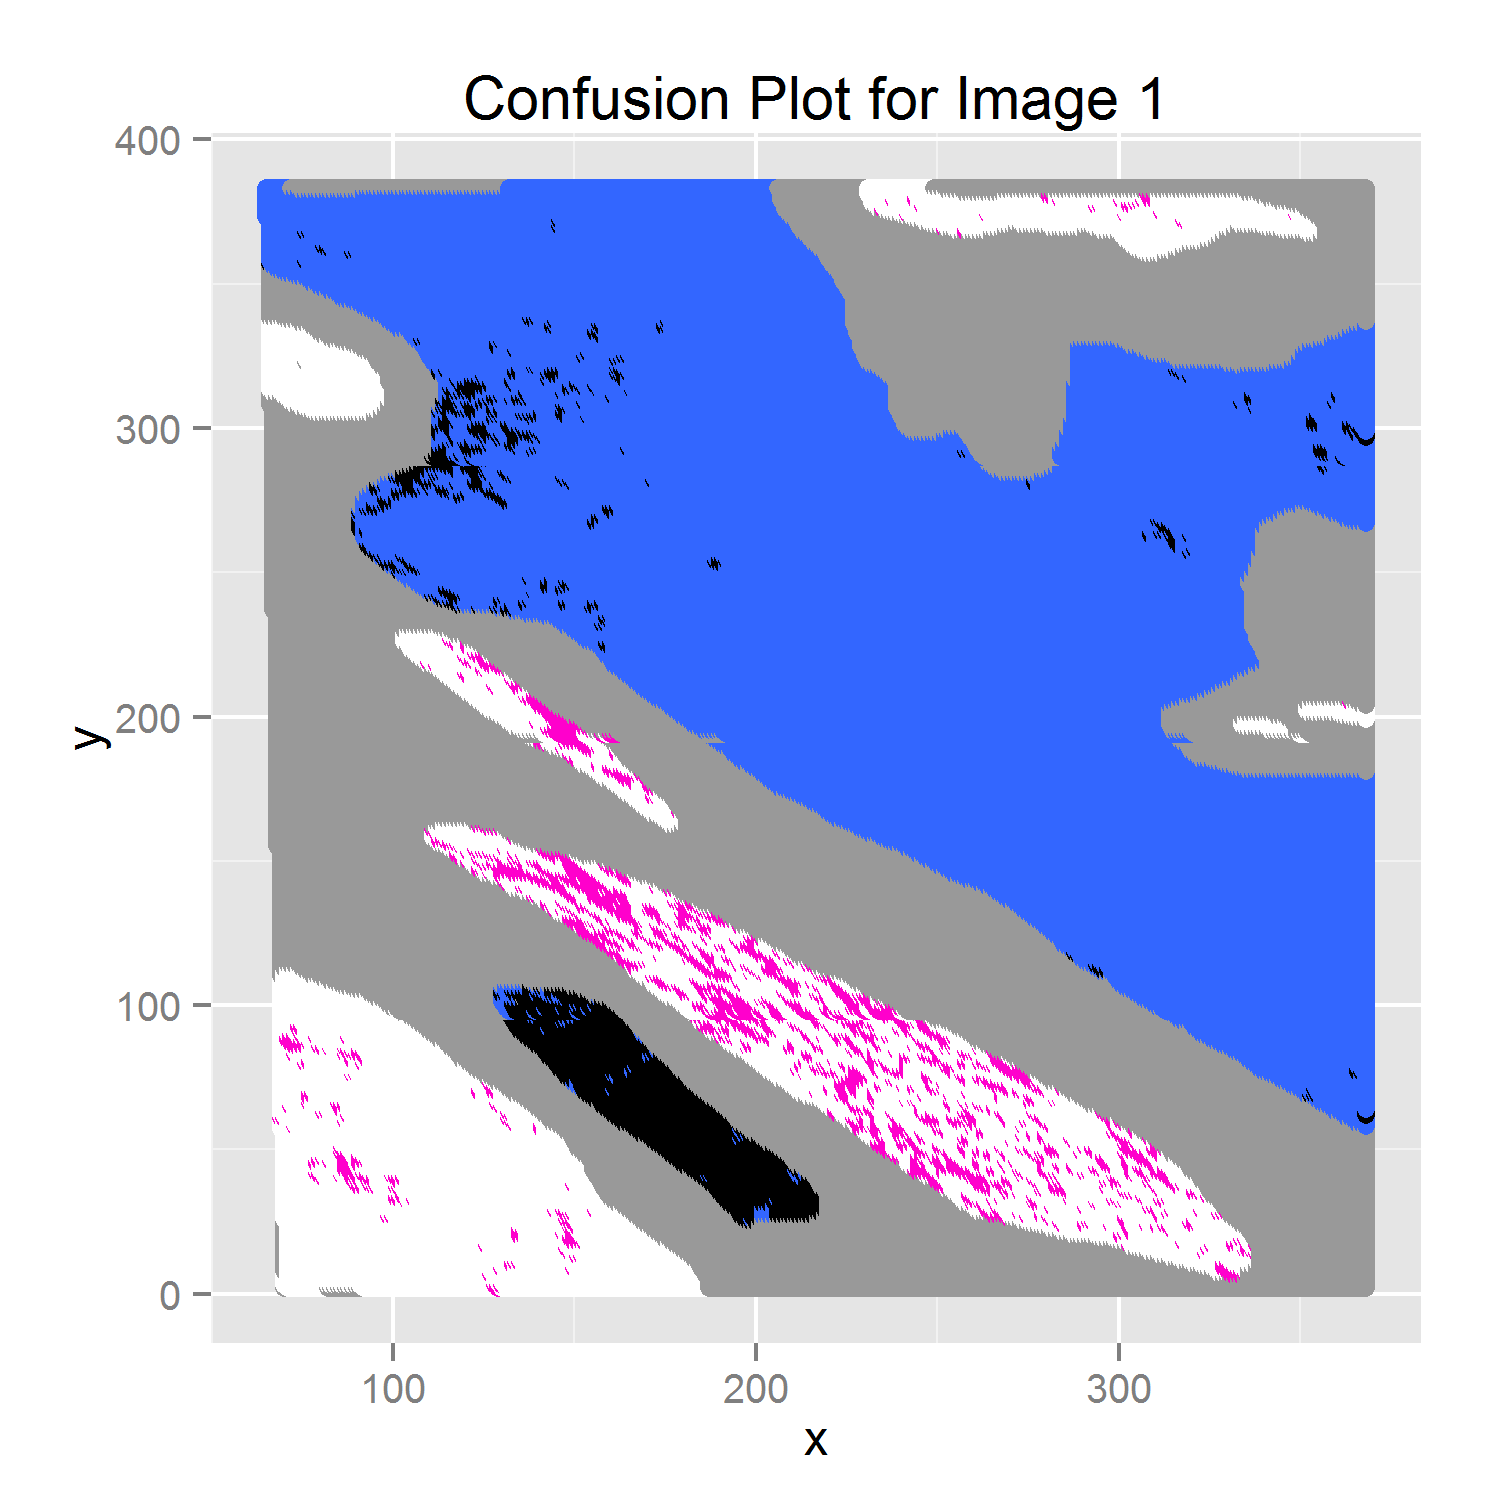
\includegraphics[width=\linewidth]{qda1_12fold_conf}
    \label{qda1_conf}
  \end{subfigure} 
  \begin{subfigure}[b]{0.3\textwidth}
    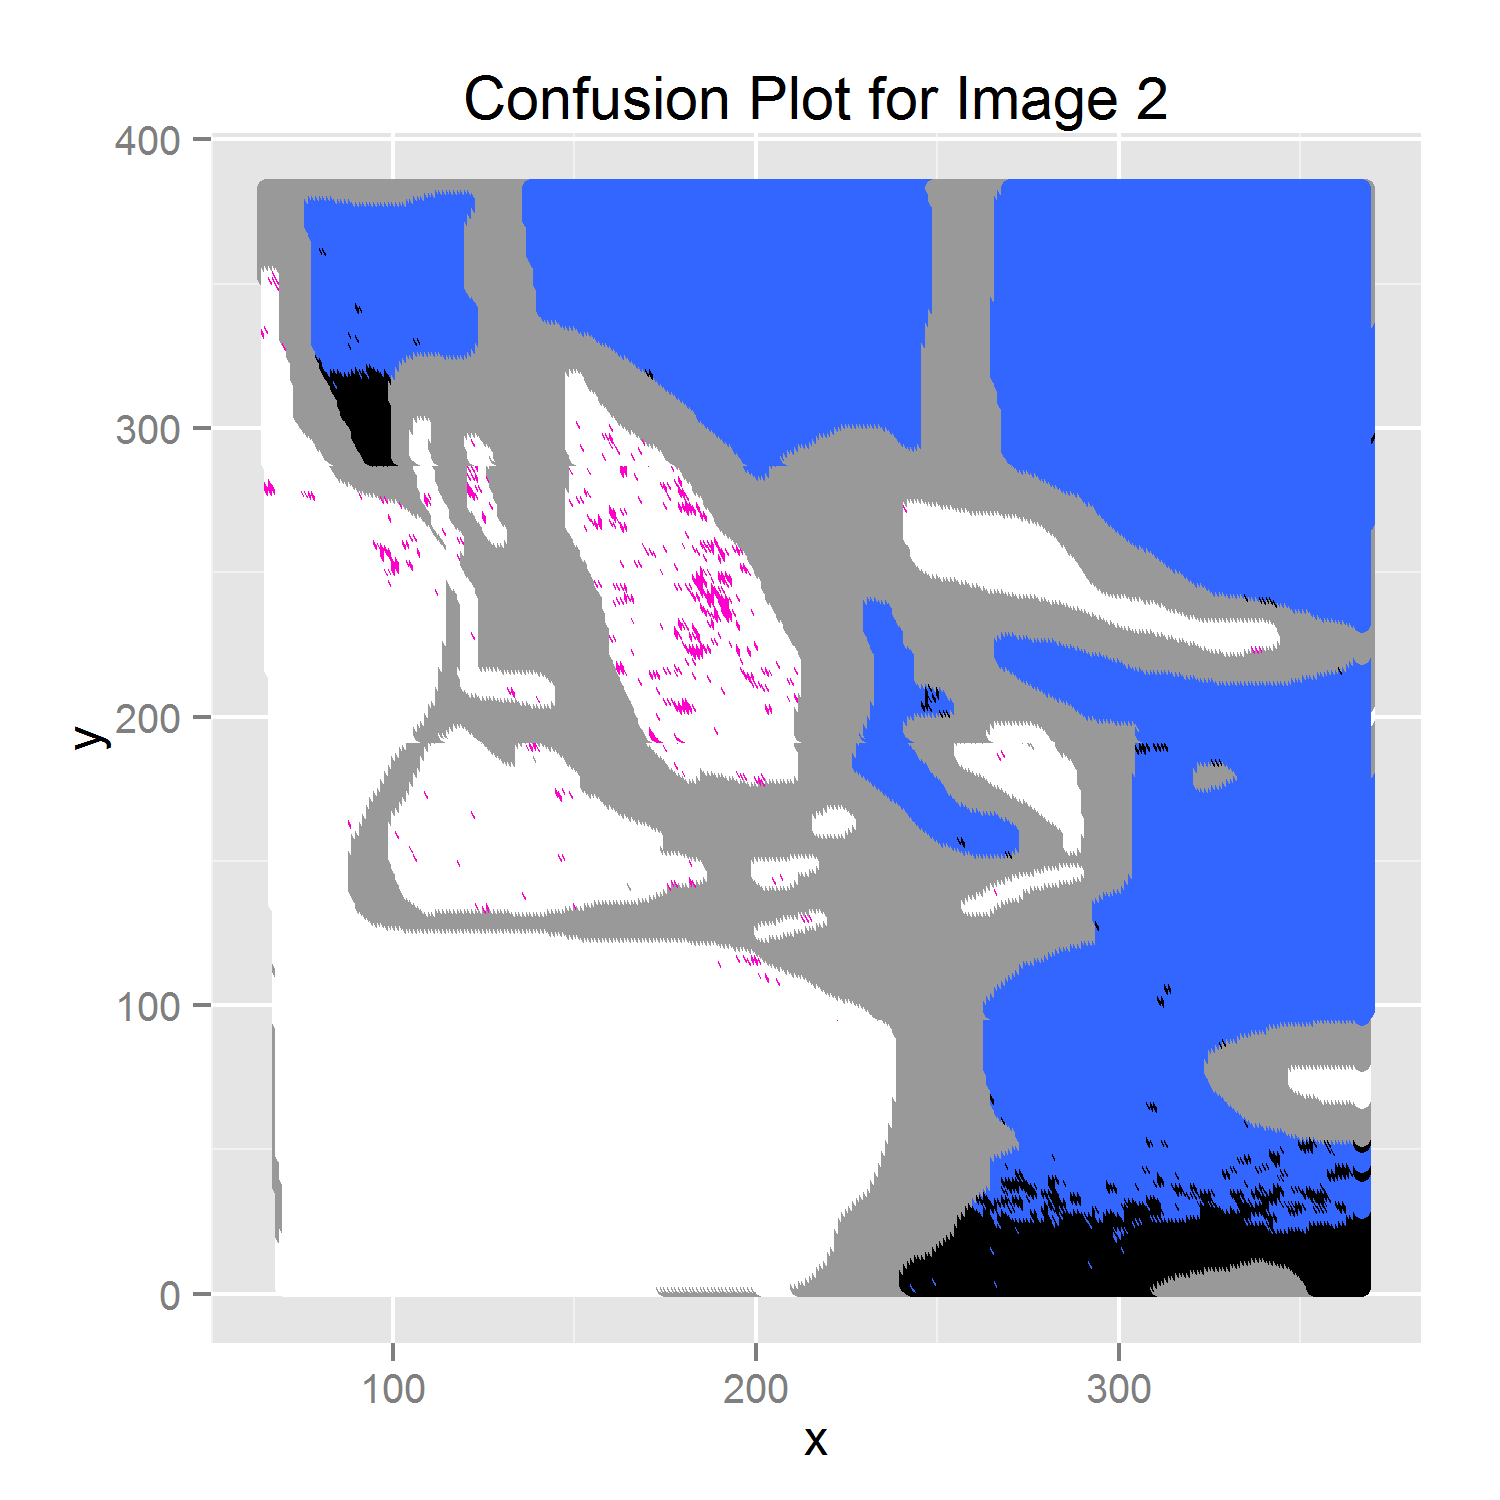
\includegraphics[width=\linewidth]{qda2_12fold_conf}
    \label{qda2_conf}
  \end{subfigure}  
  \begin{subfigure}[b]{0.3\textwidth}
    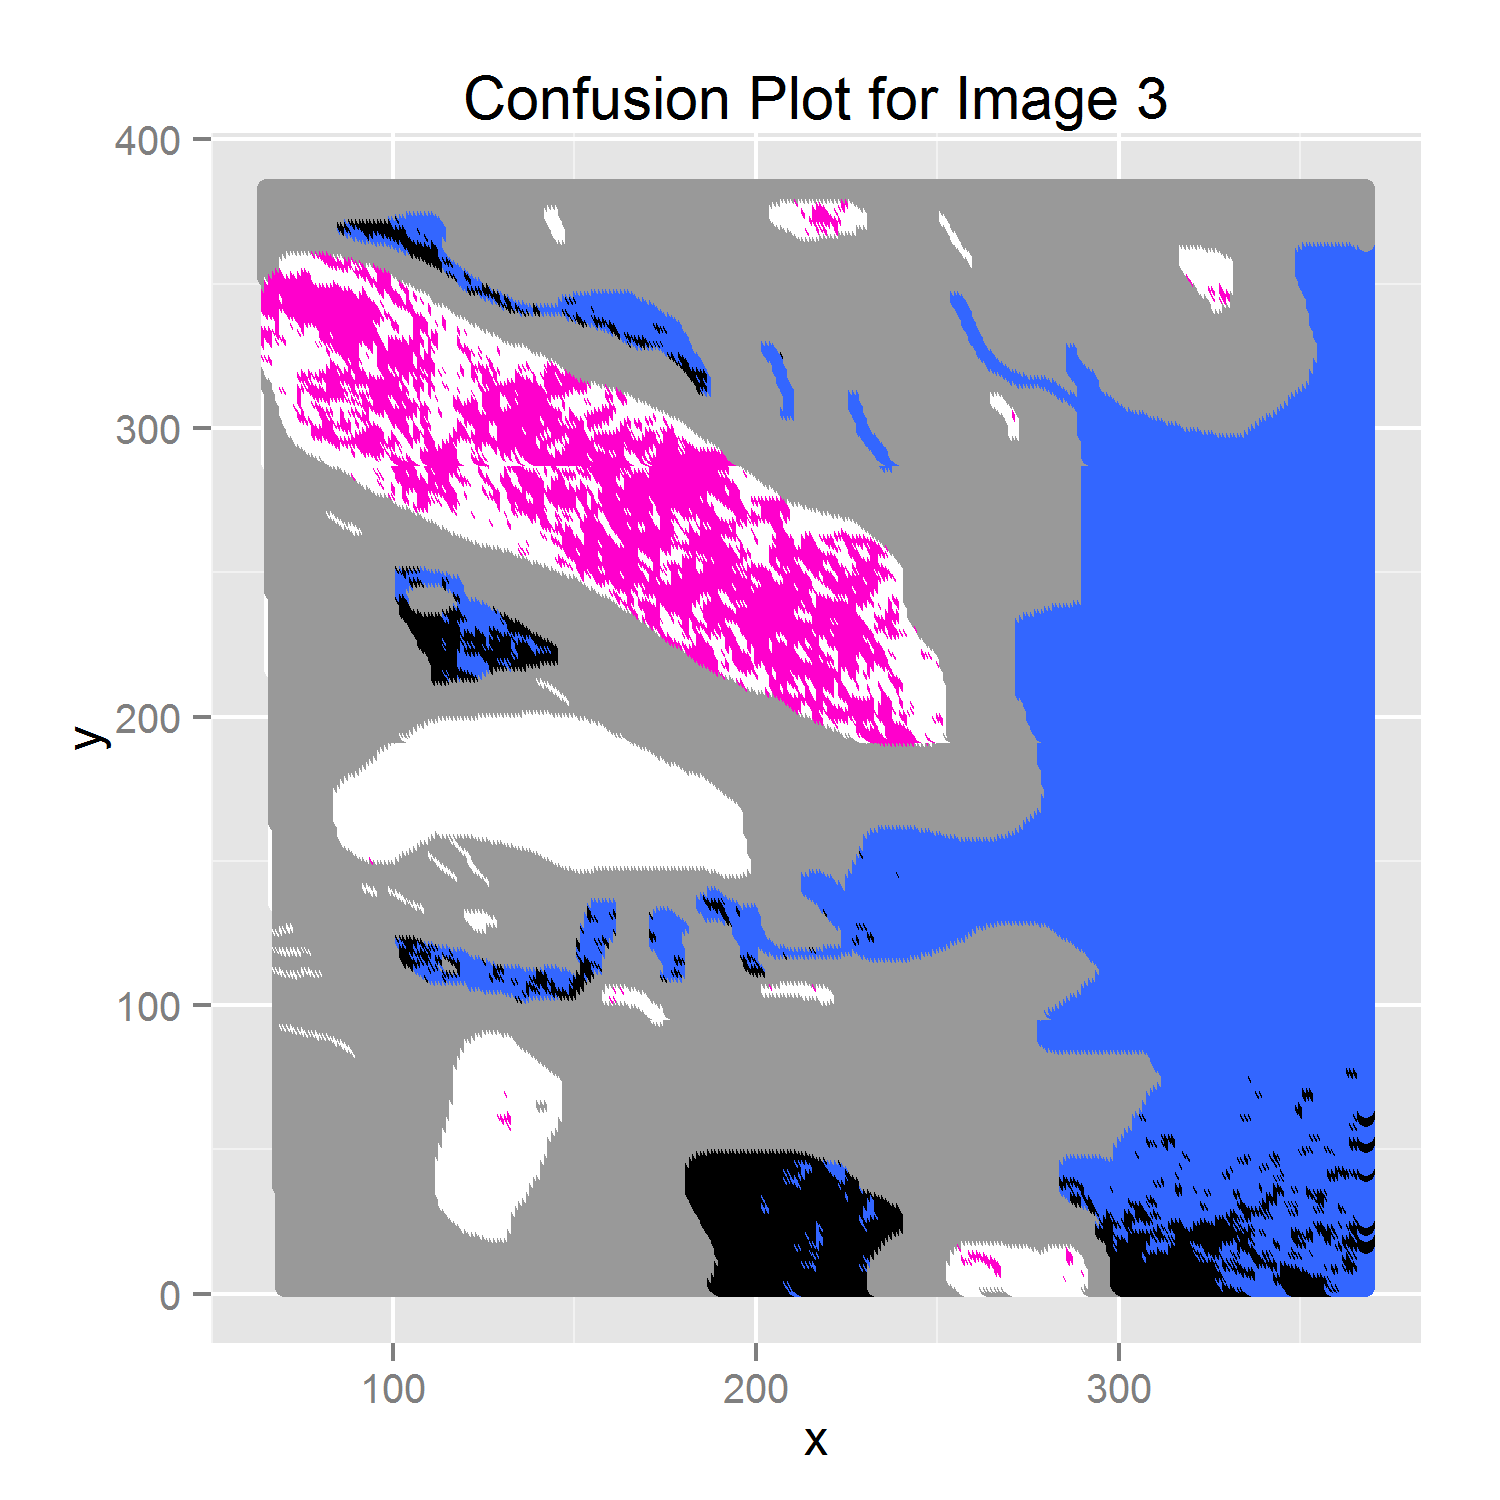
\includegraphics[width=\linewidth]{qda3_12fold_conf}
    \label{qda3_conf}
  \end{subfigure}  
  \caption{A comparison between the output of QDA and expert labels.}
  \label{fig:QDAconf}
\end{figure}

\begin{figure}[h]
  \centering 
  \begin{subfigure}[b]{0.3\textwidth}
    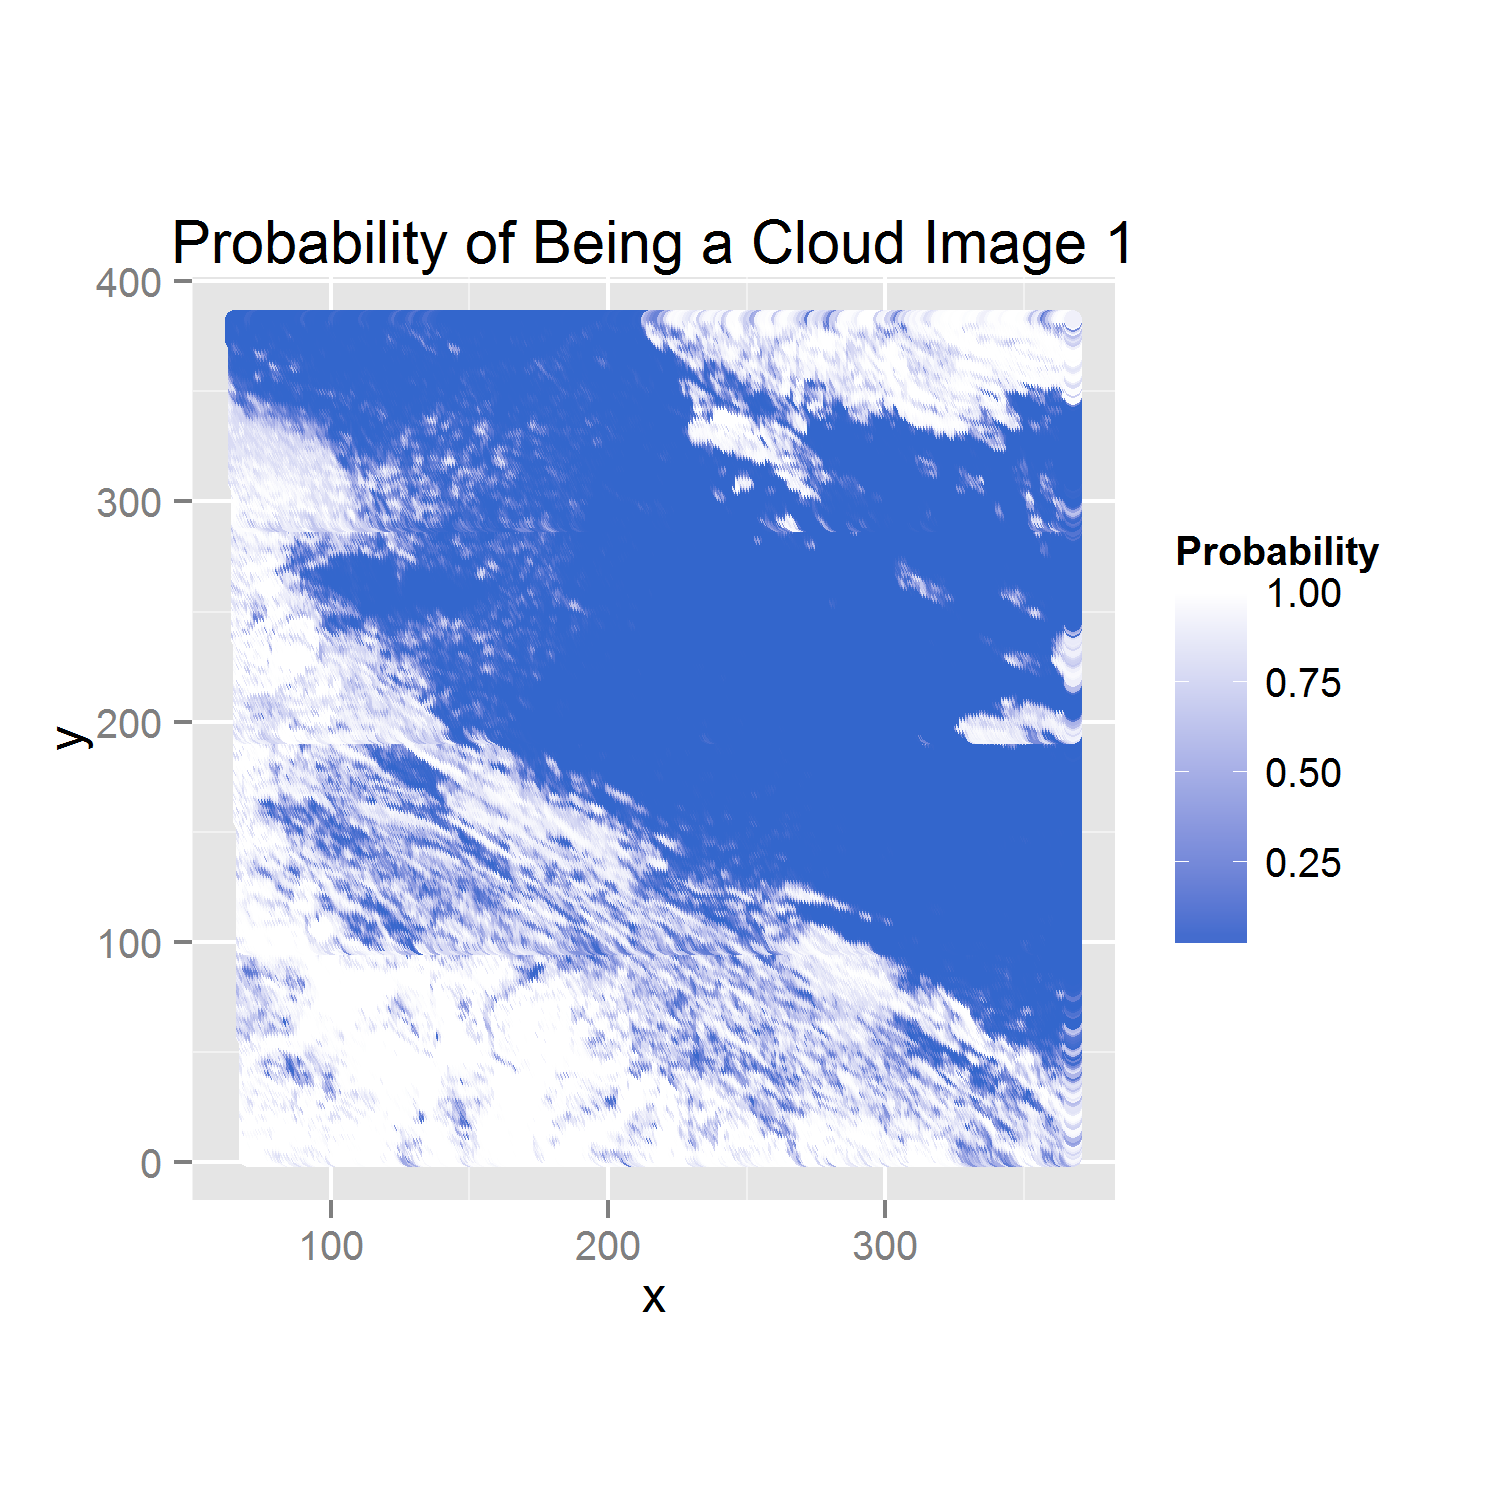
\includegraphics[width=\linewidth]{qda1_prob.png}
    \label{qda1}
  \end{subfigure} 
  \begin{subfigure}[b]{0.3\textwidth}
    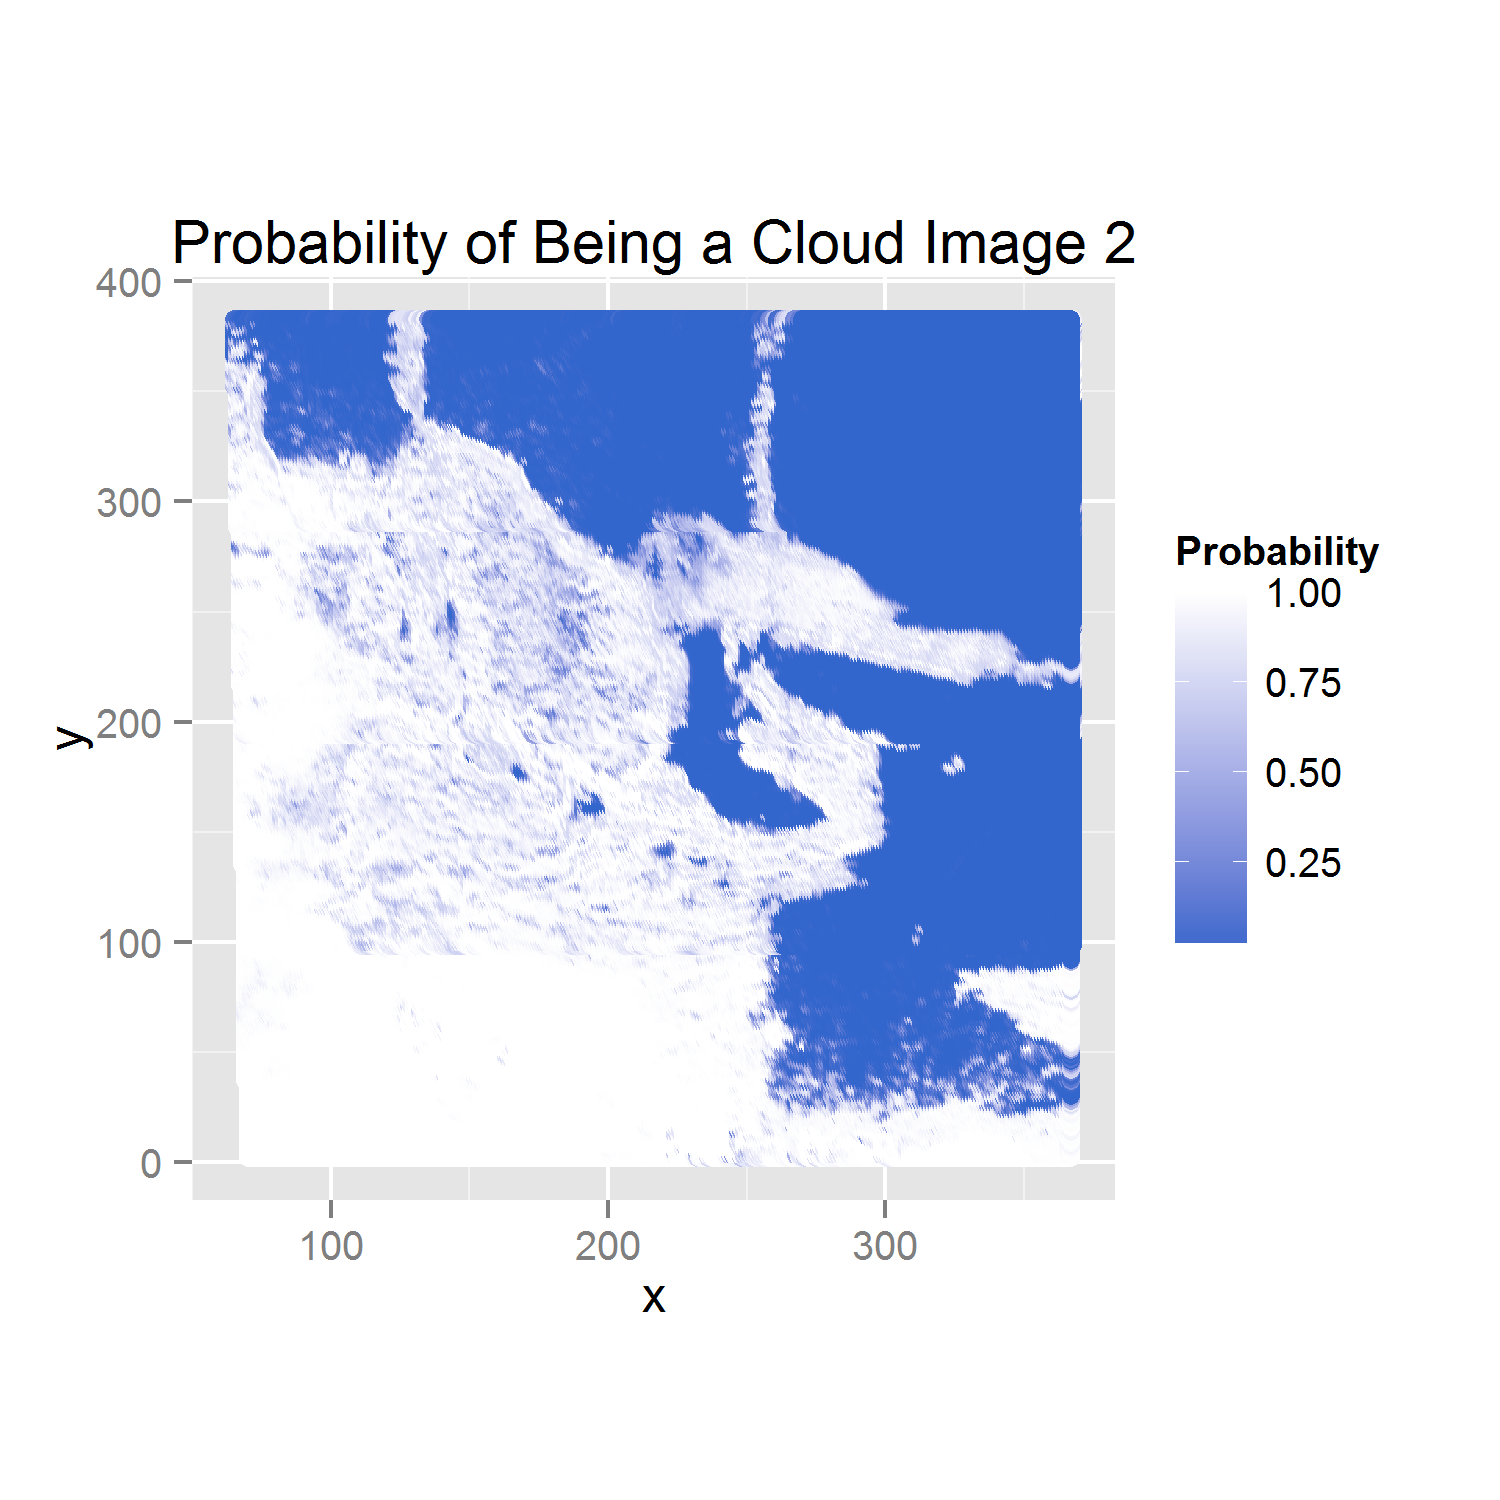
\includegraphics[width=\linewidth]{qda2_prob.png}
    \label{qda2}
  \end{subfigure}  
  \begin{subfigure}[b]{0.3\textwidth}
    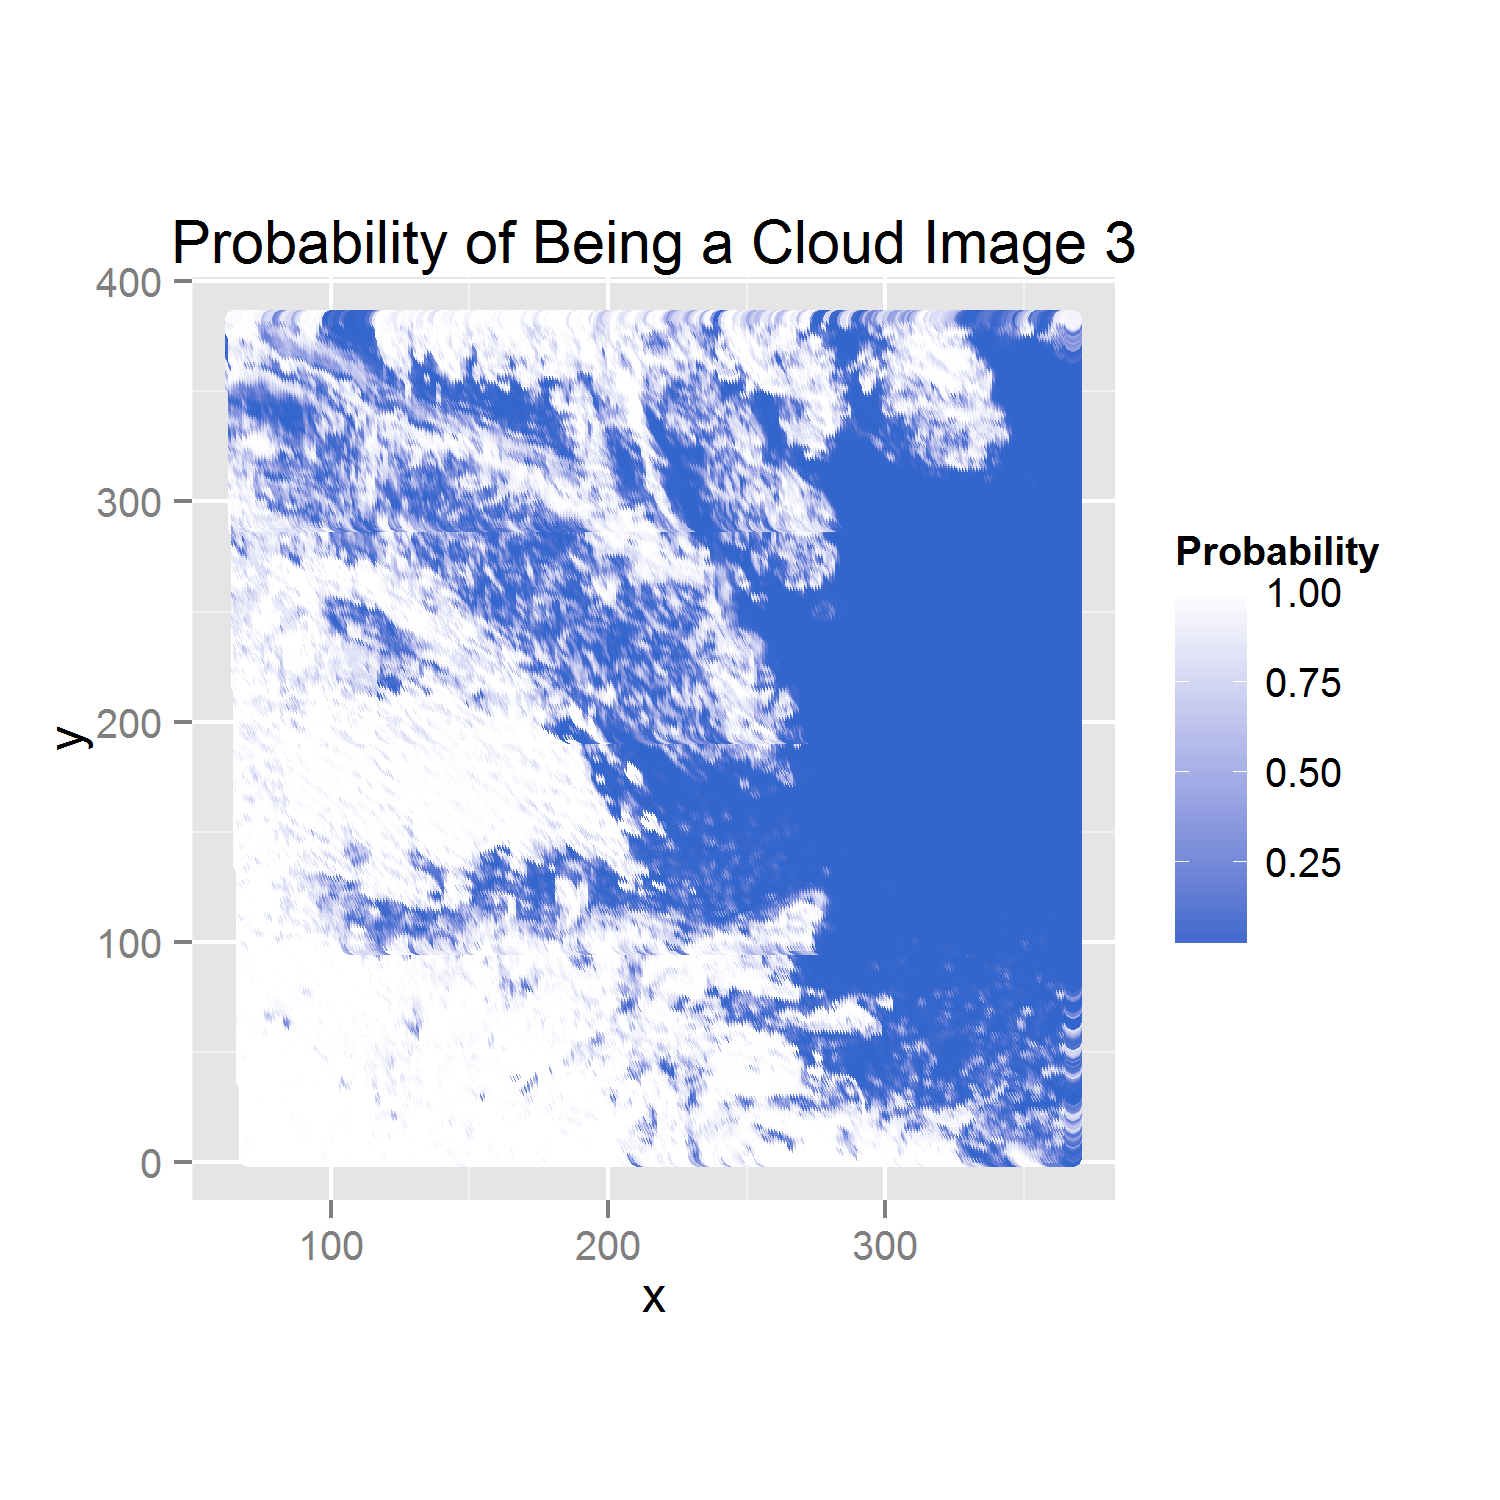
\includegraphics[width=\linewidth]{qda3_prob.png}
    \label{qda3}
  \end{subfigure}  
  \caption{Posterior probabilities of being a cloud as given by QDA}
  \label{fig:QDA}
\end{figure}

\subsection{Logit}
Logistic regression is a widely-used discriminative classification model arising from the class of generalized linear models. It is among the simplest classification methods and models the conditional distribution of the outcome given the covariates as a Bernoulli random variable with success probability given by the logistic function evaluated at $X_i \beta$, where $X_i$ is the covariate vector and $\beta$ the coefficient vector. It further supposes that the response variables are independent conditioned on the observed features. To classify, a threshold probability is chosen and all response variables with success probability above this value are labelled a success; otherwise, they are denoted as a failure. In our case, success is equivalent to cloudy and failure to clear. Preliminary results showed similar performance between the probit and logit models,  so we chose to focus on logit due its fewer assumptions (probit requires homoscedasticity and normality of errors) and greater ubiquity in practice. Use of logistic regression also assumes that the model has been properly specified with all significant and no extraneous predictors included. 

The logit model obtained via averaging after 12-fold cross-validation has $y_i = -3.356 + 1.900 * NDAI_i - 0.074 * SD_i + 9.002 * CORR_i$ where $P_i$(Cloud) = $ \frac{1}{1 + e^{-y_i}}$. To choose our cutoff value for declaring a pixel cloudy, we varied the cutoffs from .01 to 1 and calculated the misclassification error of our model at that threshold on expertly-labelled pixels. The figure below shows that the optimal threshold for this model is at .38, with an error of just under 10.1$\%$. As a consequence of this low threshold, we observe more false positives than false negatives. This will be further explored below.

Cross-validation was done by dividing each image into quandrants and holding one quadrant out for testing in each iteration of training. There were thus 12-folds in the CV procedure. We chose blocks to comprise each fold rather than a random subsample of points in order to compensate for the correlation of errors among neighboring points. The average CV error was 11.48$\%$. The ROC curve of the logit model is given in Figure 17 and has an AUC of .95.

\begin{figure}[H]
\begin{center}
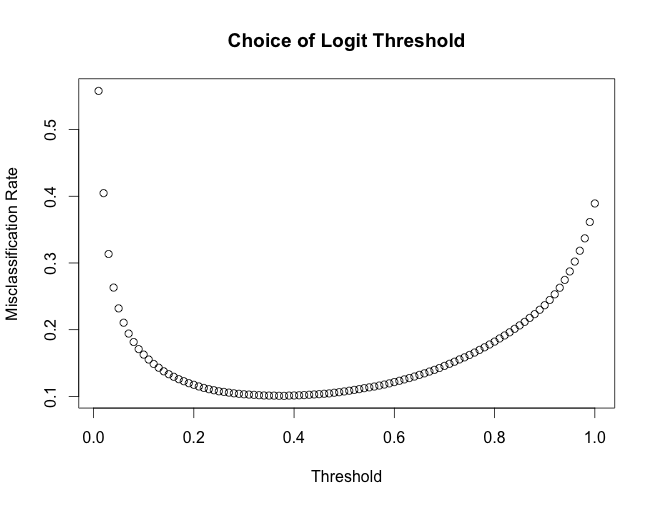
\includegraphics[scale = .35]{threshold.png}
\caption{We see a minimum in misclassification rate at .38.}
\end{center}
\end{figure}

Figure 15 gives the binary classifications overlaid on the images. Visual comparision with the expertly-labelled images suggests that we are slightly biased towards the presence of clouds as 74.2$\%$ of unlabelled points have been classified as cloudy, though this may be due to a lack of power in the expert labelling scheme.
\begin{figure}[H]
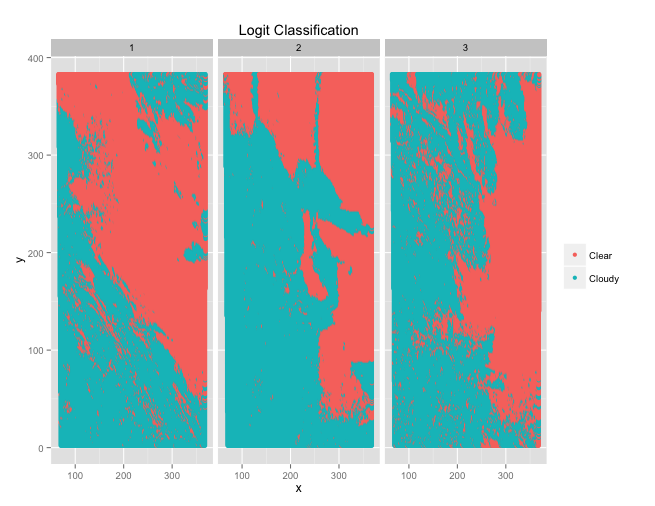
\includegraphics[width = 18cm, height = 5cm]{LogitClassification.png}
\caption{Binary classifications with threshold = .38 for logit trained via 12-fold CV.}
\end{figure}

Here we see the logit probabilites plotted spatially. This should approximate how the image would appear if the ground were not covered in snow and ice, so comparison with Figure 1 is especially appropriate. 
\begin{figure}[H]
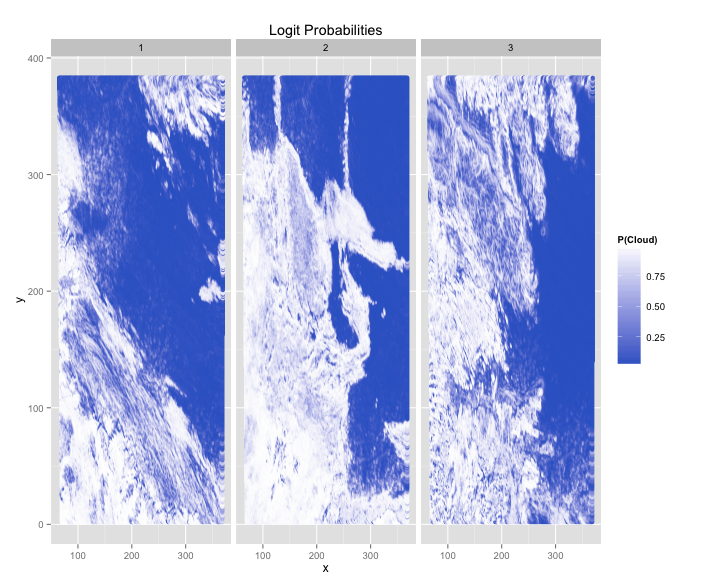
\includegraphics[width = 18cm, height = 5cm]{LogitProbabilities.png}
\caption{Probabilities for logit trained via 12-fold CV.}
\end{figure}

\begin{figure}[H]
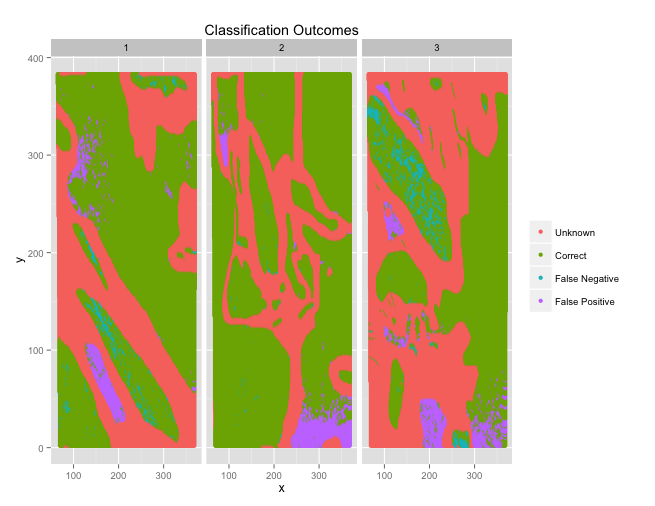
\includegraphics[width = 18cm, height = 5cm]{ClassificationOutcomes.png}
\caption{Classification results from logit with respect to the expert labels.}
\end{figure}

We now discuss the trends in misclassification. As depicted in the above figure, we have many more false positives than false negatives with large regions sometimes completely misclassified. These regions are often situated on boundaries of labelled and unlabelled points. Calculation shows the false negative rate to be 7.5$\%$ and the false positive rate to be 11.7$\%$. Models with interaction terms were considered and yielded very slight improvement as measured by drop in data-wide misclassification rate from .104 to .091. However, comparison of the misclassification plots showed that the increased complexity did not resolve the large clusters of false positives observed in each image. Especially concerning areas are the large tracts of false positives on the "island" in the southwest corner of image 1 and the southeast sections of images 2 and 3. Looking at the NDAI images only suggests these areas to be cloudy, but the AN radiance images have dark or uneven patches in these areas. Our model may thus be responding to irregularities in the ground's terrain.

\begin{figure}[h]
  \centering 
  \begin{subfigure}[b]{0.35\textwidth}
    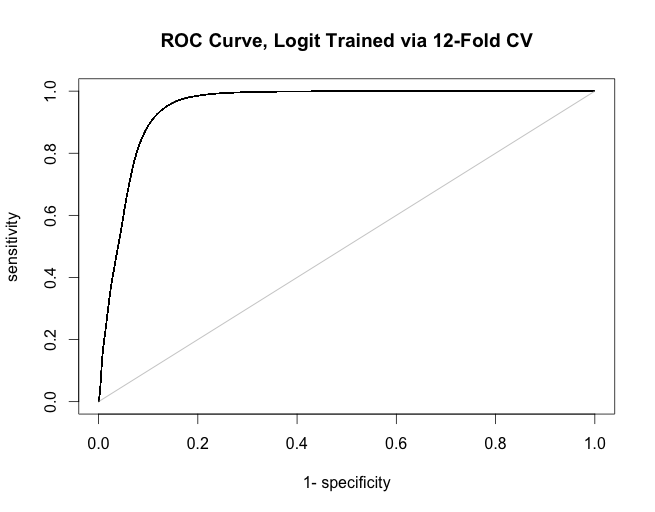
\includegraphics[width=\linewidth]{LogitROC.png}
    \label{ROC}
  \end{subfigure} 
  \begin{subfigure}[b]{0.35\textwidth}
    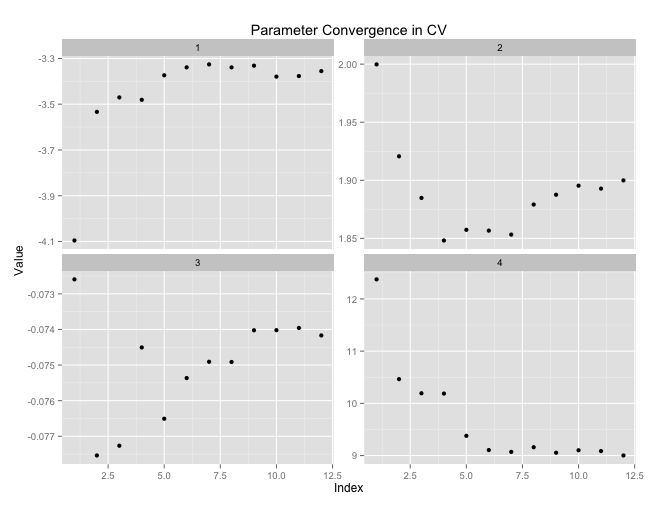
\includegraphics[width=\linewidth]{ParameterConvergence.png}
    \label{Convergence in CV}
  \end{subfigure}  
    \caption{Left: ROC Curve with AUC=.95. Right: Parameter convergence through iterations of CV. 1 - Intercept, 2 - NDAI, 3 - SD, 4 - CORR}
\end{figure}

The right half of Figure 17 displays the estimated coefficient values output by logistic regression at each stage of cross-validation. The points are a running average of the previously estimated coefficients, so we expect them to converge towards the higher iteration values. After the first few iterations for all four coefficients, we see convergent behavior, particularly for the intercept and NDAI terms. 

As found in our other models, one image outperformed the others when used as a trainer. In the case of logit, trainng on image 3 gave substantially better predictions than training on either of the other images.The AUC's were .91, .876, and .96 when training was done on image 1, 2, and 3, respectively, with associated misclassification rates .155, .204, and .096. These results inform our hypothesis that images similar to image 3 will be difficult to classify unless similar data was included in the training set. Examination illustrates that image 3 has much sharper variation in its visual features than the other two images, a phenomenon that is only partially captured by our chosen covariates. Hence we expect our predictions to be fairly accurate on images with smooth changes within cloud and ground surfaces but possibly off in regions of intense heterogeneity.

\subsection{Random Forest}

For random forest, as in all the other classifiers, we divided the three images into equal sized quadrants (2X2) rectangles in order to do 12 fold validation on the dataset.  That is, for each iteration of the validation, we dropped one of the quadrants as a test set, and trained on the remaining 11 quadrants.  Keeping the test segments as disjoint chunks from the test set ensured that our models were picking up on `higher' level structure of the dataset, and not the continuous variation of neighbouring pixels.  As such, we also expect the performance of the model on these test sets to be a much better predicator of how our model will perform on new images than if we randomly subsampled the validation folds.  Indeed, after doing random subsampling, we noticed that the AUC was at a high 0.999 for all cross validations, whereas by cross validating on the isolated quadrants, our AUC curves had much higher variance, as seen below: \\

\begin{figure}[H]
\minipage{0.2\textwidth}
  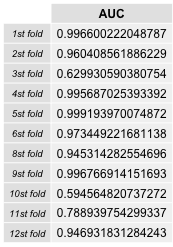
\includegraphics[width=\linewidth, height = 150pts]{AUC_12_folds.png}
\endminipage\hfill
\minipage{0.8\textwidth}%
  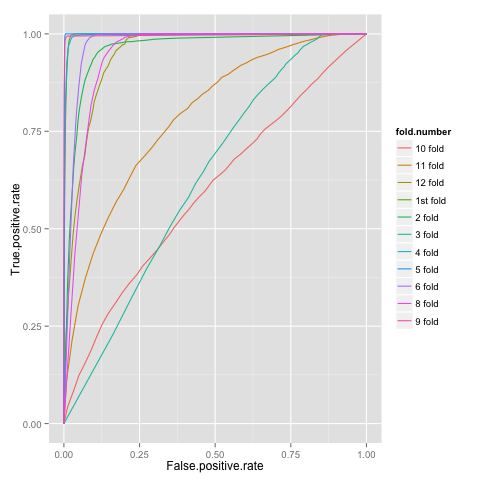
\includegraphics[width=\linewidth, height = 150pts]{ROC_fold_comparison.png}
\endminipage
  \caption{ROC across all 12 folds of quadrants}\label{}
\end{figure}

We also trained on each image and tested on the remaining two. \\


  \begin{figure}[H]
\minipage{0.5\textwidth}
\centering
  \includegraphics[width=150pts, height = 80pts ]{AUC_images.png}
\endminipage\hfill
\minipage{0.5\textwidth}
  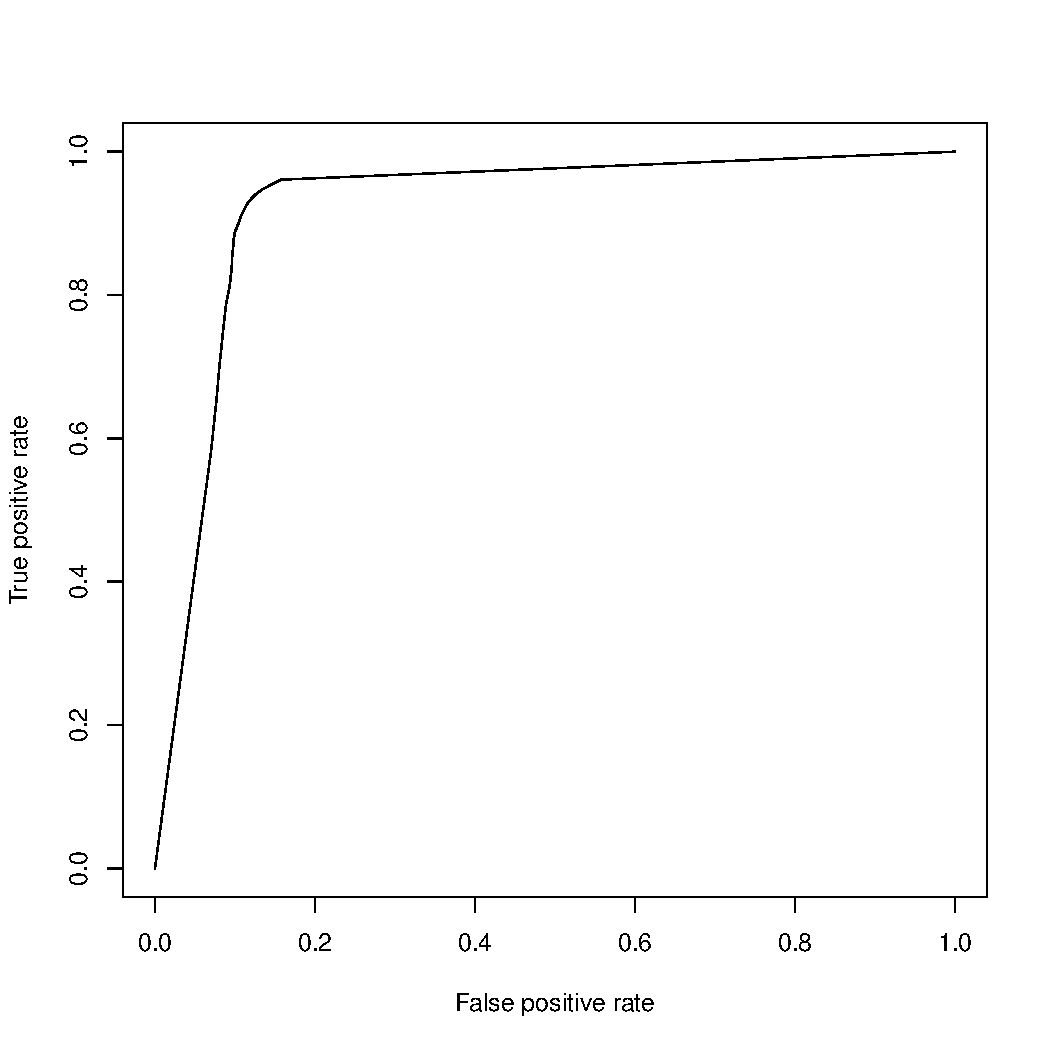
\includegraphics[width=\linewidth, height = 150pts]{ROC_image1.pdf}
\endminipage\hfill
  \caption{Convergence of ROC training on increasing number of quadrants in shuffled order}\label{}
\end{figure}

  \begin{figure}[H]
\minipage{0.5\textwidth}
  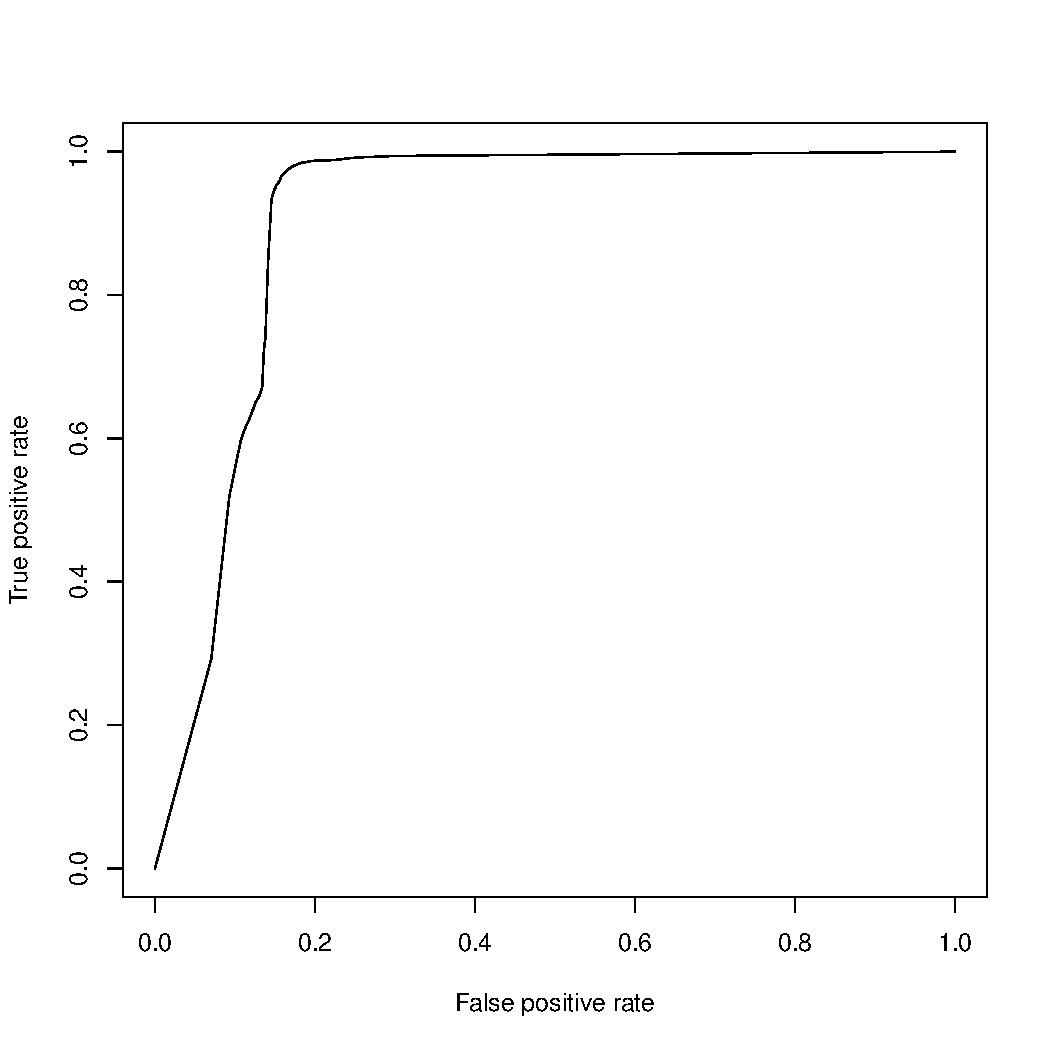
\includegraphics[width=\linewidth, height = 150pts ]{ROC_image4.pdf}
\endminipage\hfill
\minipage{0.5\textwidth}
  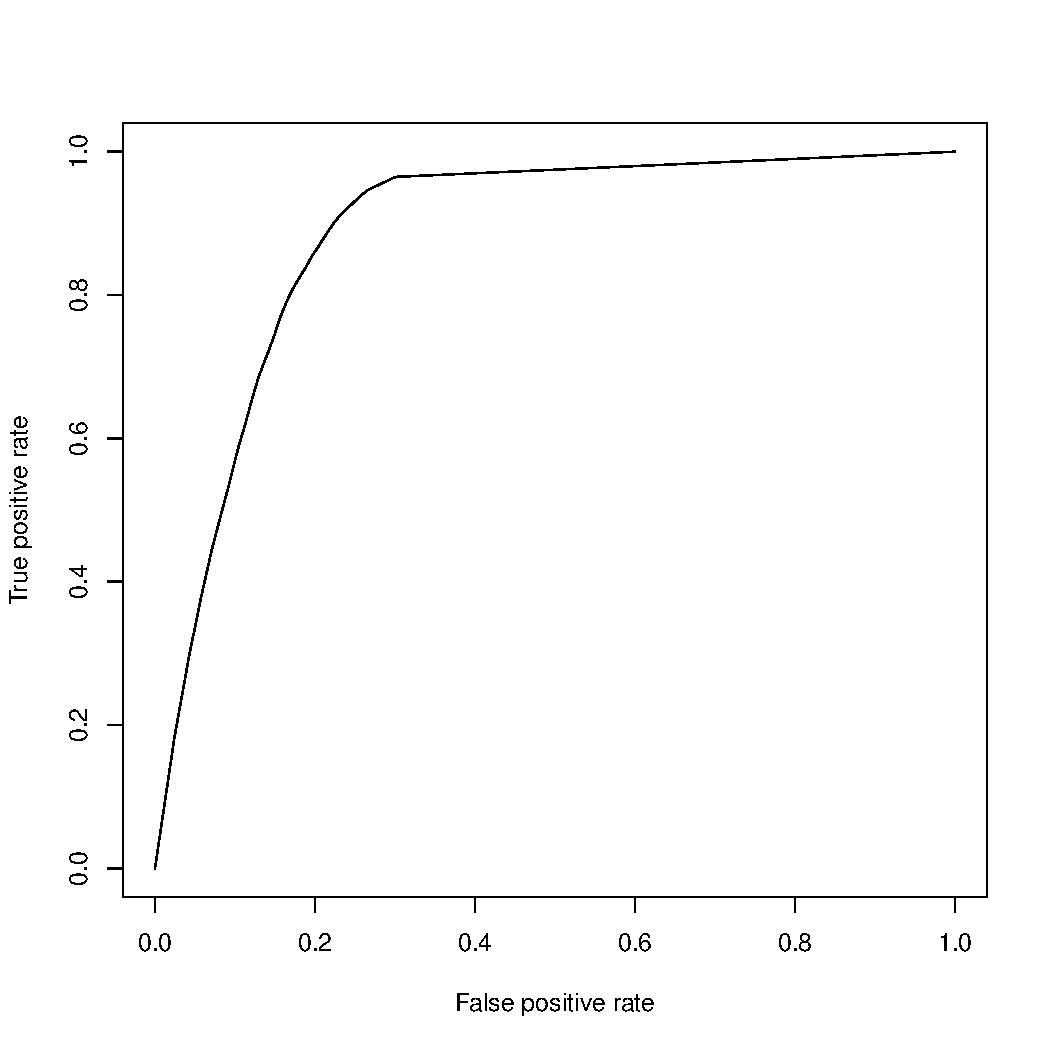
\includegraphics[width=\linewidth, height = 150pts]{ROC_image8.pdf}
\endminipage\hfill
  \caption{Convergence of ROC training on increasing number of quadrants in shuffled order}\label{}
\end{figure}


 To test convergence, one of the things we did was increase the training set from including 1 quadrant, to including 2 quadrants, up to including 11 quadrants (using the complement as the test set).  For each of the 3 aforementioned classes of training, we trained on a range of forest sizes, from 2 trees to 50. It was interesting to note that the continuity of increasing the training set by neighbouring quadrants displayed much less convergence than by increasing the training quadrant set in a randomly subsampled way.  The following three plots make this clear.  In the first case....\\

\begin{figure}[H]
\minipage{0.5\textwidth}
  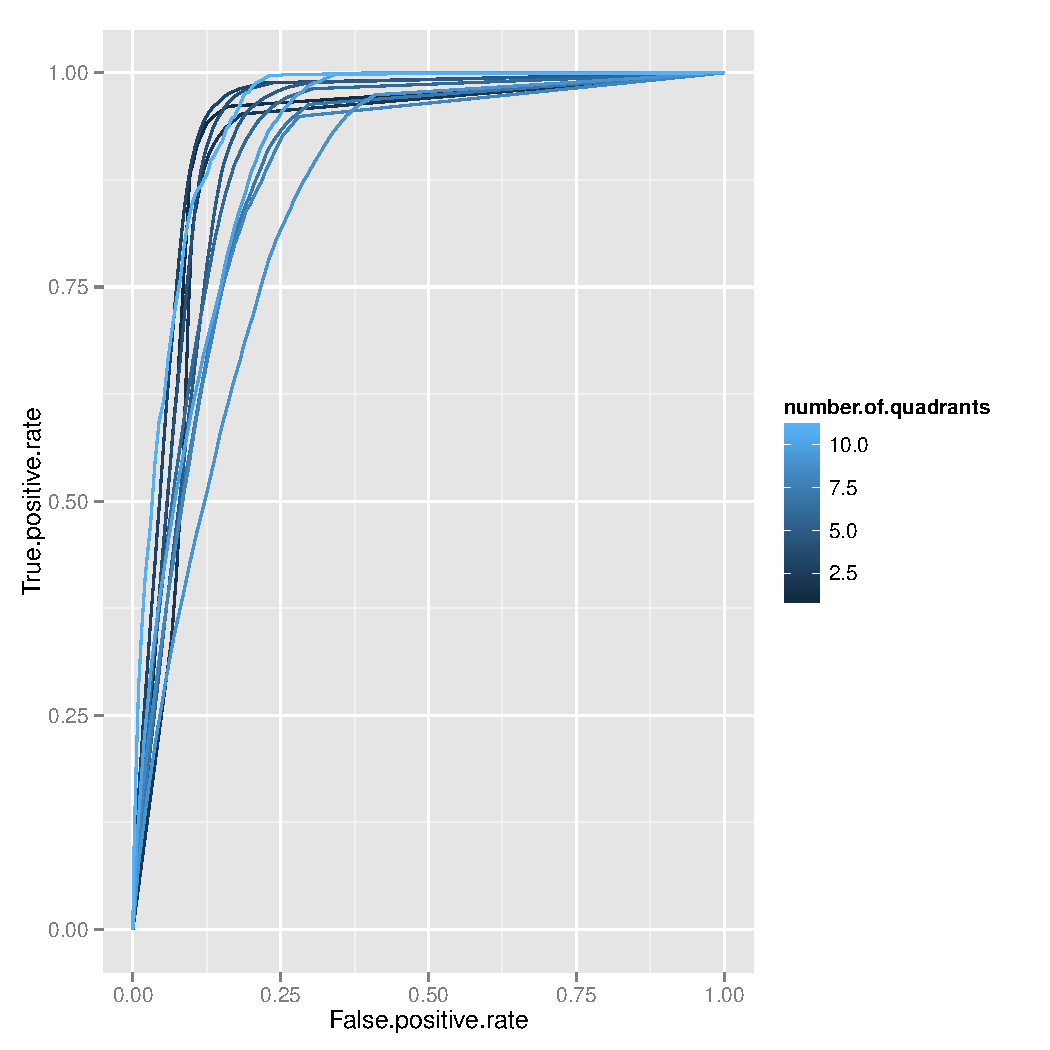
\includegraphics[width=\linewidth, height = 180pts]{ROC_converge1.pdf}
    \caption{Convergence of ROC training on increasing number of quadrants}\label{}
\endminipage
\minipage{0.5\textwidth}

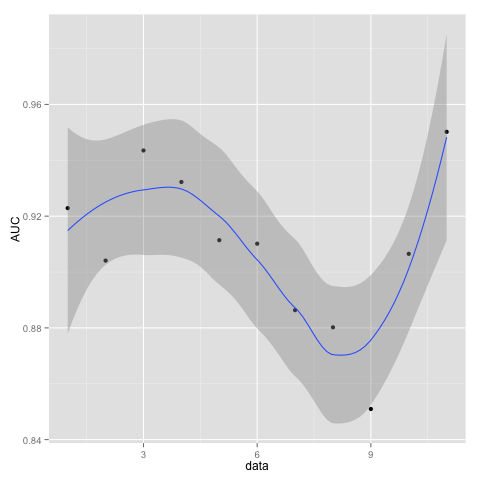
\includegraphics[width=\linewidth, height = 180pts]{AUCconverge.png}
  \caption{Smoothed convergence of AUC for growing training set 50 trees and 3 features}\label{}
\endminipage

  \end{figure}
  
  \begin{figure}[H]
\minipage{0.5\textwidth}
  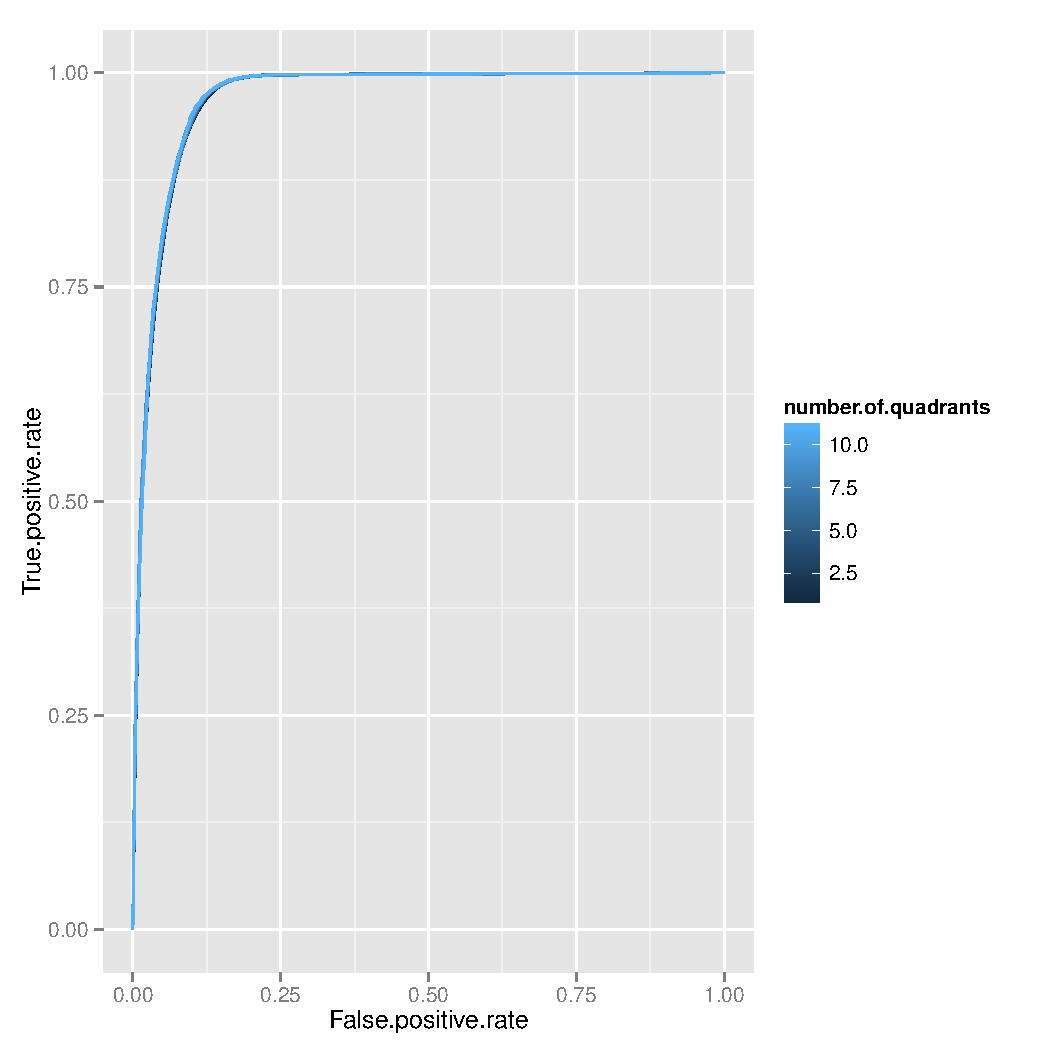
\includegraphics[width=\linewidth, height = 180pts ]{ROC_converge_shuffle1.pdf}
\endminipage\hfill
\minipage{0.5\textwidth}
  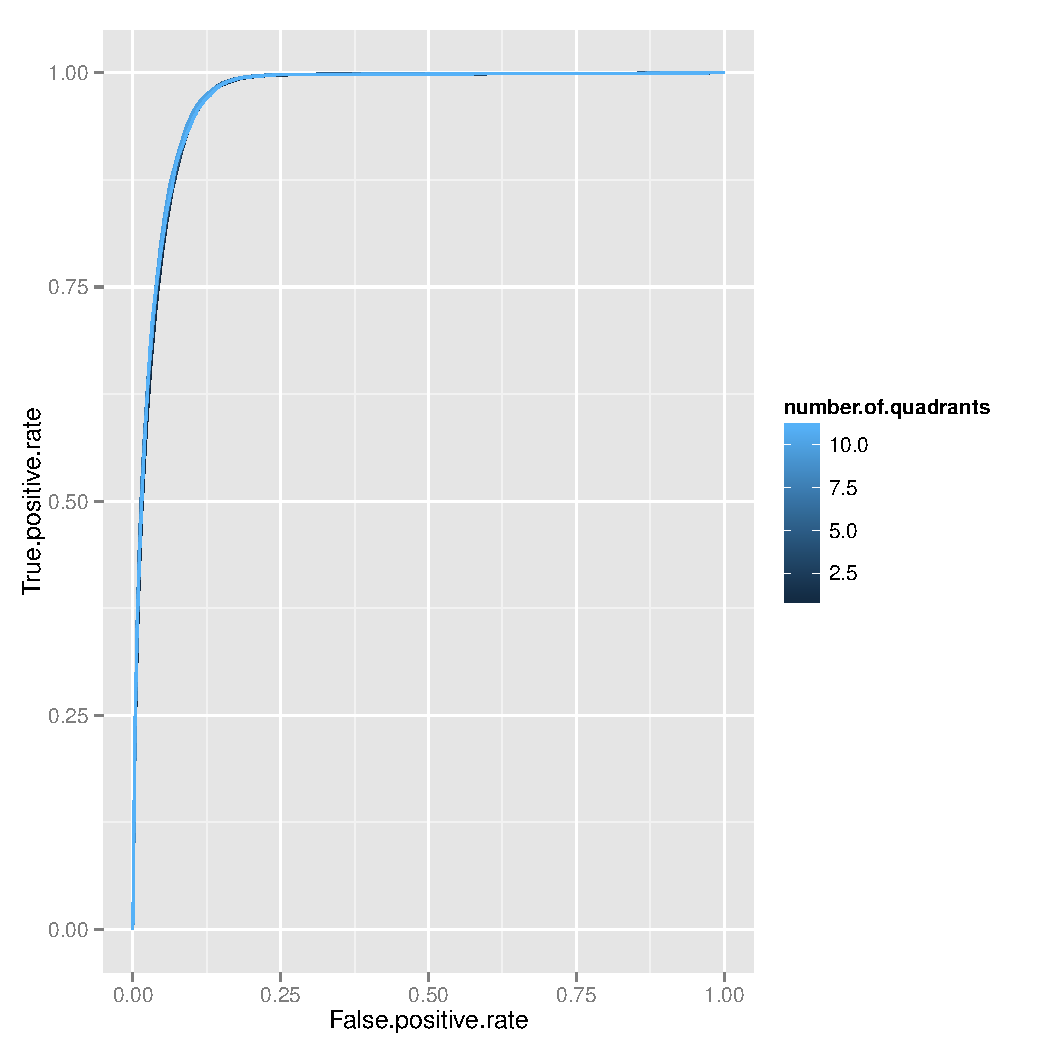
\includegraphics[width=\linewidth, height = 180pts]{ROC_converge_shuffle2.pdf}
\endminipage\hfill
  \caption{Convergence of ROC training on increasing number of quadrants in shuffled order}\label{}
\end{figure}
  
To gather a quantitative measurement of the importance of each feature, we first ran random forest using all the features and looked at the GIni importance measure.  This is calculated by recording the difference between the Gini measure of a random forest's predictions on a fold and the Gini measure with a particular feature's values randomly shuffled.  The intuition is that if a feature were crucial to the forest's trees, than randomly shuffling that feature will drastically decrease it's Gini measure.  Sure enough, NDAI, SD and CORR   consistently ranked as the clear top three in all cross validations. \\

  \begin{figure}[H]
\minipage{0.4\textwidth}
  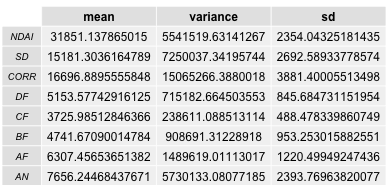
\includegraphics[width=\linewidth, height = 140pts ]{Gini_mean_sd.png}
\endminipage\hfill
\minipage{0.6\textwidth}
  \includegraphics[width=\linewidth, height = 180pts]{Gini_importance.png}
\endminipage\hfill
  \caption{Gini importance measures across folds}\label{}
\end{figure}

{\bf Where was the model performing poorly?}

  \begin{figure}[H]
\minipage{0.5\textwidth}
  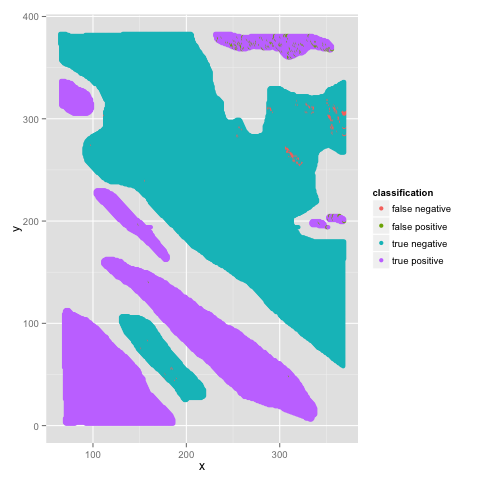
\includegraphics[width=\linewidth, height = 180pts ]{classification_1.png}
\endminipage\hfill
\minipage{0.5\textwidth}
  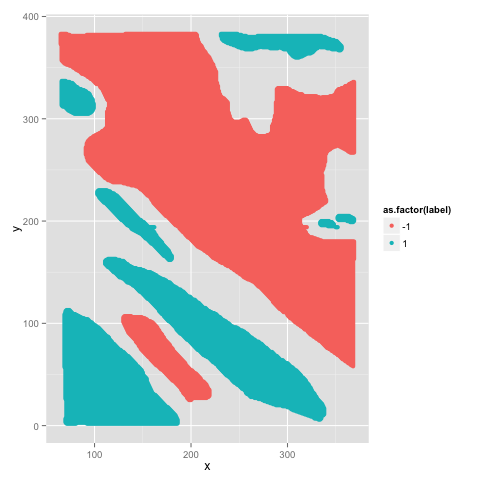
\includegraphics[width=\linewidth, height = 180pts]{label_1.png}
\endminipage\hfill
\end{figure}

  \begin{figure}[H]
\minipage{0.5\textwidth}
  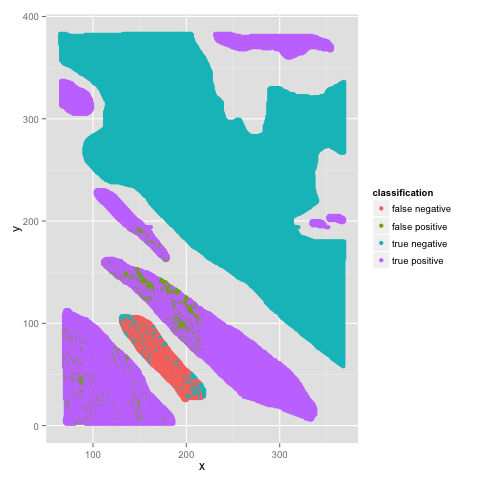
\includegraphics[width=\linewidth, height = 180pts ]{classification_3.png}
\endminipage\hfill
\minipage{0.5\textwidth}
  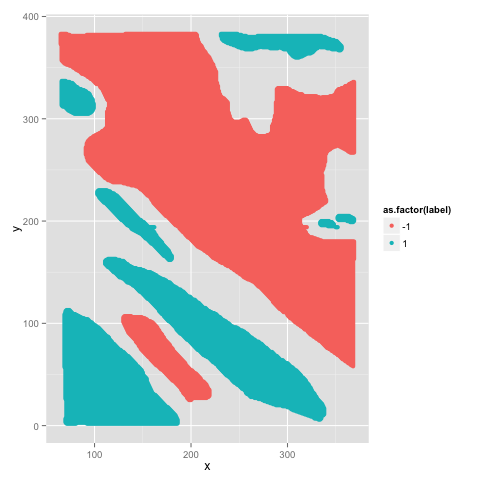
\includegraphics[width=\linewidth, height = 180pts]{label_3.png}
\endminipage\hfill
\end{figure}

\begin{figure}[H]
\minipage{0.5\textwidth}
  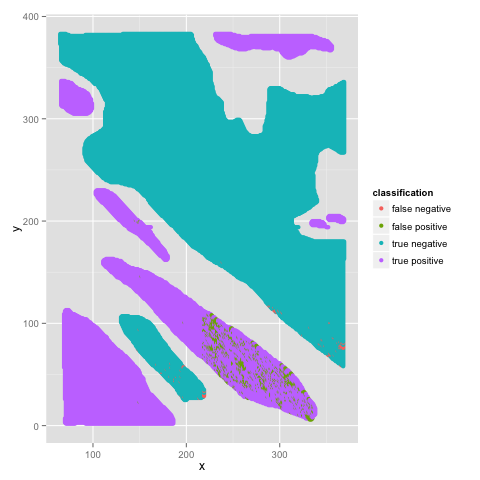
\includegraphics[width=\linewidth, height = 180pts ]{classification_4.png}
\endminipage\hfill
\minipage{0.5\textwidth}
  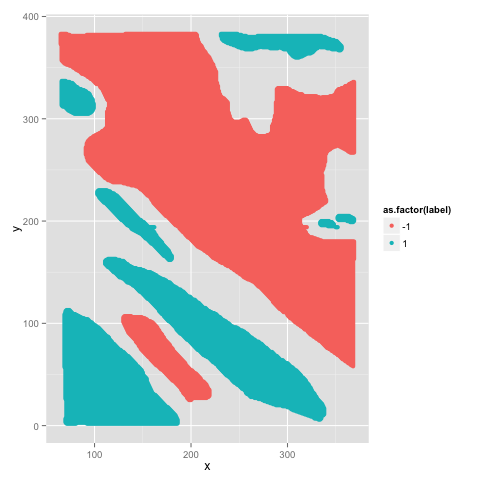
\includegraphics[width=\linewidth, height = 180pts]{label_4.png}
\endminipage\hfill
\end{figure}


\begin{figure}[H]
\minipage{0.5\textwidth}
  \includegraphics[width=\linewidth, height = 180pts ]{classification_9.png}
\endminipage\hfill
\minipage{0.5\textwidth}
  \includegraphics[width=\linewidth, height = 180pts]{label_9.png}
\endminipage\hfill
\end{figure}

  \begin{figure}[H]
\minipage{0.5\textwidth}
  \includegraphics[width=\linewidth, height = 180pts ]{classification_10.png}
\endminipage\hfill
\minipage{0.5\textwidth}
  \includegraphics[width=\linewidth, height = 180pts]{label_10.png}
\endminipage\hfill
\end{figure}

\begin{figure}[H]
\minipage{0.5\textwidth}
  \includegraphics[width=\linewidth, height = 180pts ]{classification_11.png}
\endminipage\hfill
\minipage{0.5\textwidth}
  \includegraphics[width=\linewidth, height = 180pts]{label_11.png}
\endminipage\hfill
\end{figure}


\section{Reproducibility}

{\bf How we organized out code and github repo}


 \begin{thebibliography}{1}

\bibitem{notes} Ben-Hur, A., Elisseeff, A., Guyon, I.: A stability based method for discovering structure in clustered data. In: Pacific Symposium on Biocomputing, pp. 6�17.   
\end{thebibliography}


\end{document}